%%%%%%%%%%%%%%%%%%%%%%%%%%%%%%%%%%%%%%%%%%%%%%%%%%%%%%%%%%%%
%%% ELIFE ARTICLE TEMPLATE
%%%%%%%%%%%%%%%%%%%%%%%%%%%%%%%%%%%%%%%%%%%%%%%%%%%%%%%%%%%%
%%% PREAMBLE 
\documentclass[9pt,lineno]{elife}
% Use the onehalfspacing option for 1.5 line spacing
% Use the doublespacing option for 2.0 line spacing
% Please note that these options may affect formatting.
% Additionally, the use of the \newcommand function should be limited.

\usepackage{lipsum} % Required to insert dummy text
\usepackage[version=4]{mhchem}
\usepackage{fancyvrb}
\usepackage{siunitx}
\DeclareSIUnit\Molar{M}

%%%%%%%%%%%%%%%%%%%%%%%%%%%%%%%%%%%%%%%%%%%%%%%%%%%%%%%%%%%%
%%% ARTICLE SETUP
%%%%%%%%%%%%%%%%%%%%%%%%%%%%%%%%%%%%%%%%%%%%%%%%%%%%%%%%%%%%
\title{An engineered biosensor enables dynamic aspartate measurements in living cells}

\author[1,2,\authfn{1}]{Kristian Davidsen}
\author[3,\authfn{1}*]{Jonathan S Marvin}
\author[3]{Timothy A Brown}
\author[1*]{Lucas B Sullivan}
\affil[1]{Human Biology Division, Fred Hutchinson Cancer Center, Seattle, WA, USA}
\affil[2]{Molecular and cellular biology program, University of Washington, Seattle, WA, USA}
\affil[3]{Howard Hughes Medical Institute (HHMI), Janelia Research Campus, Ashburn, VA, USA}

\corr{marvinj@janelia.hhmi.org}{JSM}
\corr{sullivan@fredhutch.org}{LBS}

\contrib[\authfn{1}]{These authors contributed equally to this work}

%%%%%%%%%%%%%%%%%%%%%%%%%%%%%%%%%%%%%%%%%%%%%%%%%%%%%%%%%%%%
%%% ARTICLE START
%%%%%%%%%%%%%%%%%%%%%%%%%%%%%%%%%%%%%%%%%%%%%%%%%%%%%%%%%%%%

\begin{document}

\maketitle

\begin{abstract}
Intracellular levels of the amino acid aspartate are responsive to changes in metabolism in mammalian cells and can correspondingly alter cell function, highlighting the need for robust tools to measure aspartate abundance.
However, comprehensive understanding of aspartate metabolism has been limited by the throughput, cost, and static nature of the mass spectrometry based measurements that are typically employed to measure aspartate levels.
To address these issues, we have developed a GFP-based sensor of aspartate (iASPSnFR2), where the fluorescence intensity corresponds to aspartate concentration.
As a purified protein, \textit{in vitro}, the sensor has a 20-fold increase in fluorescence upon aspartate saturation, with dose dependent fluorescence changes covering a physiologically relevant intracellular aspartate concentration range and no significant off target binding.
Expressed in mammalian cell lines, sensor intensity correlated with aspartate levels determined by mass spectrometry and could resolve temporal changes in intracellular aspartate using both genetic and pharmacological manipulations.
These data demonstrate the utility of iASPSnFR2 and highlight the opportunities it provides for temporally resolved and high throughput applications of variables that affect aspartate levels.
\end{abstract}


\section{Introduction}
The primary tool used by metabolism researchers, liquid chromatography coupled with mass spectrometry (LCMS), involves extracting pools of thousands of cells and measuring the liberated metabolites.
This approach is powerful but has significant drawbacks; it requires highly specialized equipment, it is expensive for use, and sample preparation by chemical extractions homogenizes metabolic differences that may occur amongst different cells in complex samples or across subcellular compartments.
Metabolite extraction also consumes precious samples that might otherwise be desirable to analyze over time or with additional outputs.
Development of genetically encoded protein sensors (biosensors) over the past two decades has provided new opportunities to visualize the release, production, and depletion of important signaling molecules and metabolites with subsecond and subcellular resolution (reviewed in \cite{Kostyuk2019-qc, Koveal2020-cl}).
Thus, biosensors provide a solution to many of the problems with metabolite extraction and LCMS, with the trade off of monitoring only one metabolite per sensor.

Aspartate is amongst the most concentrated metabolites in cells \citep{Park2016-ap}, yet it is one of only two amino acids that is not predominantly acquired from the environment.
While the other, glutamate, is made from glutamine by the enzyme glutaminase, no analogous enzyme exists in humans to convert asparagine to aspartate \citep{Sullivan2018-gz}.
Instead, aspartate must be synthesized by transamination of the tricarboxylic acid (TCA) cycle metabolite oxaloacetate by the cytosolic enzyme GOT1 or the mitochondrial enzyme GOT2.
Notably, aspartate synthesis can occur from multiple metabolic sources \textit{via} complex metabolic reactions occurring in the cytosol and mitochondria, rendering aspartate levels at the whole cell and subcellular levels dependent on multiple metabolic variables.
For example, impairments to mitochondrial respiration can deplete aspartate levels and aspartate restoration can reestablish proliferation in cells with defective mitochondria \citep{Sullivan2015-xf, Birsoy2015-pg, Cardaci2015-xy, Hart2023-gp}.
Alterations to aspartate levels are associated with modifications to cell function in multiple biological processes, including stem cells \citep{Tournaire2022-ut, Arnold2022-ft}, immune cells \citep{Bailis2019-mf}, endothelial cells \citep{Diebold2019-hh}, and cancer \citep{Helenius2021-ht}.
In addition, genetic methods to elevate intracellular aspartate can impact biology \textit{in vivo}, increasing tumor growth \citep{Sullivan2018-gz, Garcia-Bermudez2018-mj} and improving hematopoietic function \citep{Qi2021-jv}.
Therefore, our understanding of metabolism in multiple biological systems could be improved with the availability of an aspartate biosensor.

We have previously developed a biosensor for glutamate using the \textit{E.coli} glutamate/aspartate binding domain GltI linked to circularly permutated GFP (iGluSnFR) \citep{Marvin2013-qq}, and subsequently optimized it by modulating its affinity, kinetics, color, and total fluorescence change (SF-iGluSnFR and iGluSnFR3) \citep{Marvin2018-ks, Aggarwal2023-pi}.
Since GltI domain also binds, aspartate, albeit at lower affinity than glutamate  \citep{Hu2008-nd}, we reasoned that subtle modifications to the ligand binding site could switch the relative aspartate/glutamate specificity.
We achieved this using a small mutagenesis screen on a precursor to iGluSnFR3, guided by the crystal structure of glutamate-bound GltI.
The resulting biosensor, iASPSnFR2, was characterized \textit{in vitro} and in cells with matched LCMS determination of aspartate, showing that it accurately reports genetic and pharmacological manipulation of intracellular aspartate.




\section{Results}

\subsection{Protein engineering}
We observed that the original iGluSnFR bound both glutamate and aspartate, with higher affinity for the former \citep{Marvin2013-qq}.
To shift the relative affinities of the two ligands, we looked at the structure of the binding pocket  \citep{Hu2008-nd}, and sampled all possible amino acid substitutions of residue S72, which interacts with the side-chain carboxylate of bound glutamate.
By expressing mutant sensors in bacteria and measuring the fluorescence of bacterial lysate in response to aspartate or glutamate, we identified S72A and S72P as having switched specificity from glutamate to aspartate.
S72T, identified in a faster version of iGluSnFR \citep{Helassa2018-fb} also preferably binds aspartate over glutamate.

As an improved glutamate sensor (iGluSnFR3) was being developed \citep{Aggarwal2023-pi}, we took a variant from that process and queried the effect of S72A, S72T, and S72P on aspartate/glutamate affinity.
In bacterial cell lysate, S72P maintained the expected shift to a preference for aspartate, and had a higher fluorescence fold increase (∆F/F) than either S72A or S72T.
To further increase specificity, we sampled mutations at S27, which also interacts the carboxylate of bound glutamate, in the background of S72P.
One of those, S27A, had lower affinity for glutamate while mostly maintaining affinity for aspartate (\FIGSUPP[Fig1]{f1S1}, panel A).
We then moved forward with this variant and named it iASPSnFR2.
Since we expected to be using this sensor in cell culture studies, and potentially \textit{in vivo}, over the course of hours or even days, we added a C-terminal red fluorescence protein, mRuby3, to enable correction for expression and movement artefacts.
All biochemical characterization is reported with iASPSnFR2.mRuby3 and for iASPSnFR2 signal normalization in cells we used a mix of iASPSnFR2.mRuby3 and nuclear expressed RFP.

The sensor is yellow-shifted in excitation and emission compared to typical GFP-based sensors, since its chromophore is formed by the triad of GYG and has the T203Y pi-stacking mutations of the Venus yellow fluorescent protein.
% Does this^ need a citation or figure reference? 
This yellow-shift will facilitate observation deeper into tissues using 2-photon microscopy, as the sensor has high ∆F/F and significant 2-photon cross-section at 1040 nm (\FIGSUPP[Fig1]{f1S1}, panel B).
It has a Kd for aspartate of about 50 µM and binds glutamate and asparagine with Kd greater than 5 mM (\FIG{Fig1}, panel B).
It does not appreciably change its green fluorescence in response to other amino acids (\FIGSUPP[Fig1]{f1S2}, panel A).
Surprisingly, the mRuby3 component responds to amino acids at high millimolar concentrations, indicating a non-specific effect (potentially interacting with the C-terminal histidine tag) (\FIGSUPP[Fig1]{f1S2}, panel B), although this increase in fluorescence is still an order of magnitude lower than the green fluorescence response and at amino acid concentrations that are unlikely to be achieved in most cell types.
The sensor also does not robustly respond to other decoys considered relevant to aspartate metabolism nor to relevant pharmacological treatments (\FIGSUPP[Fig1]{f1S2}, panel C).
It is sensitive to pH, as are all cpGFP-based sensors, but changes in fluorescence due to changes in aspartate far exceed what one might expect from changes in fluorescence due to changes in pH (\FIGSUPP[Fig1]{f1S2}, panel E).
Unlike a recently reported and concurrently developed sensor for aspartate \citep{Hellweg2023}, which has a lower maximum ∆F/F at 37˚C than at 30˚C, our aspartate sensor has the same maximum ∆F/F at 37°C as it does st 30˚C, which is slightly higher than its maximum ∆F/F at 23°C (\FIGSUPP[Fig1]{f1S2}, panel D).


\begin{figure}[ht!]
\centering
\fbox{\includegraphics[width=0.68\linewidth]{figures/Fig1.pdf}}
\caption{
Protein engineering and \textit{in vitro} characterization.
(A) Structure of the binding pocket of glutamate-bound GltI (2VHA.pdb) with residues S72 (left) and S27 (right) shown as sticks and bound glutamate as sticks inside transparent spheres.
(B) Fluorescence response of purified iASPSnFR2.mRuby3 when titrated with aspartate (black) or glutamate or asparagine (grey tones).
Ex. 485 nm (20 nm bandpass), Em. 535 nm (20 nm bandpass).
Error bars are s.d. of three technical replicates.
(C) Live cell imaging in the phase contrast, GFP and RFP channels of H1299 Nuclear-RFP cells expressing iASPSnFR2 after 24h with/without glutamine.
}
\label{fig:Fig1}
\figsupp[Aspartate specificity and excitation/emission spectra.]{
(A) Switching specificity of an iGluSnFR3 precursor from glutamate to aspartate using S72X library (left) and S72P, S27X library (right).
Titrations with aspartate (solid lines) and glutamate (dashed lines) in bacterial lysate.
(B) Excitation and emission spectra of iASPSnFR2.mRuby3.
Left, 1-photon spectra.
Excitation wavelength was varied from 400 nm to 520 nm (7.5 nm bandpass) while observing emission at 535 nm (10 nm bandpass).
Emission wavelength was varied from 535 nm to 600 nm (10 nm bandpass) while exciting at 510 nm (7.5 nm bandpass).
Fluorescence was measured in the both the absence (dashed lines) and presence of 10 mM aspartate (solid lines).
Right, 2-photon cross-sections, also ± 10 mM aspartate, with an overlay of calculated ∆F/F (green).
Vertical bar indicates 1040 nm.
}{\fbox{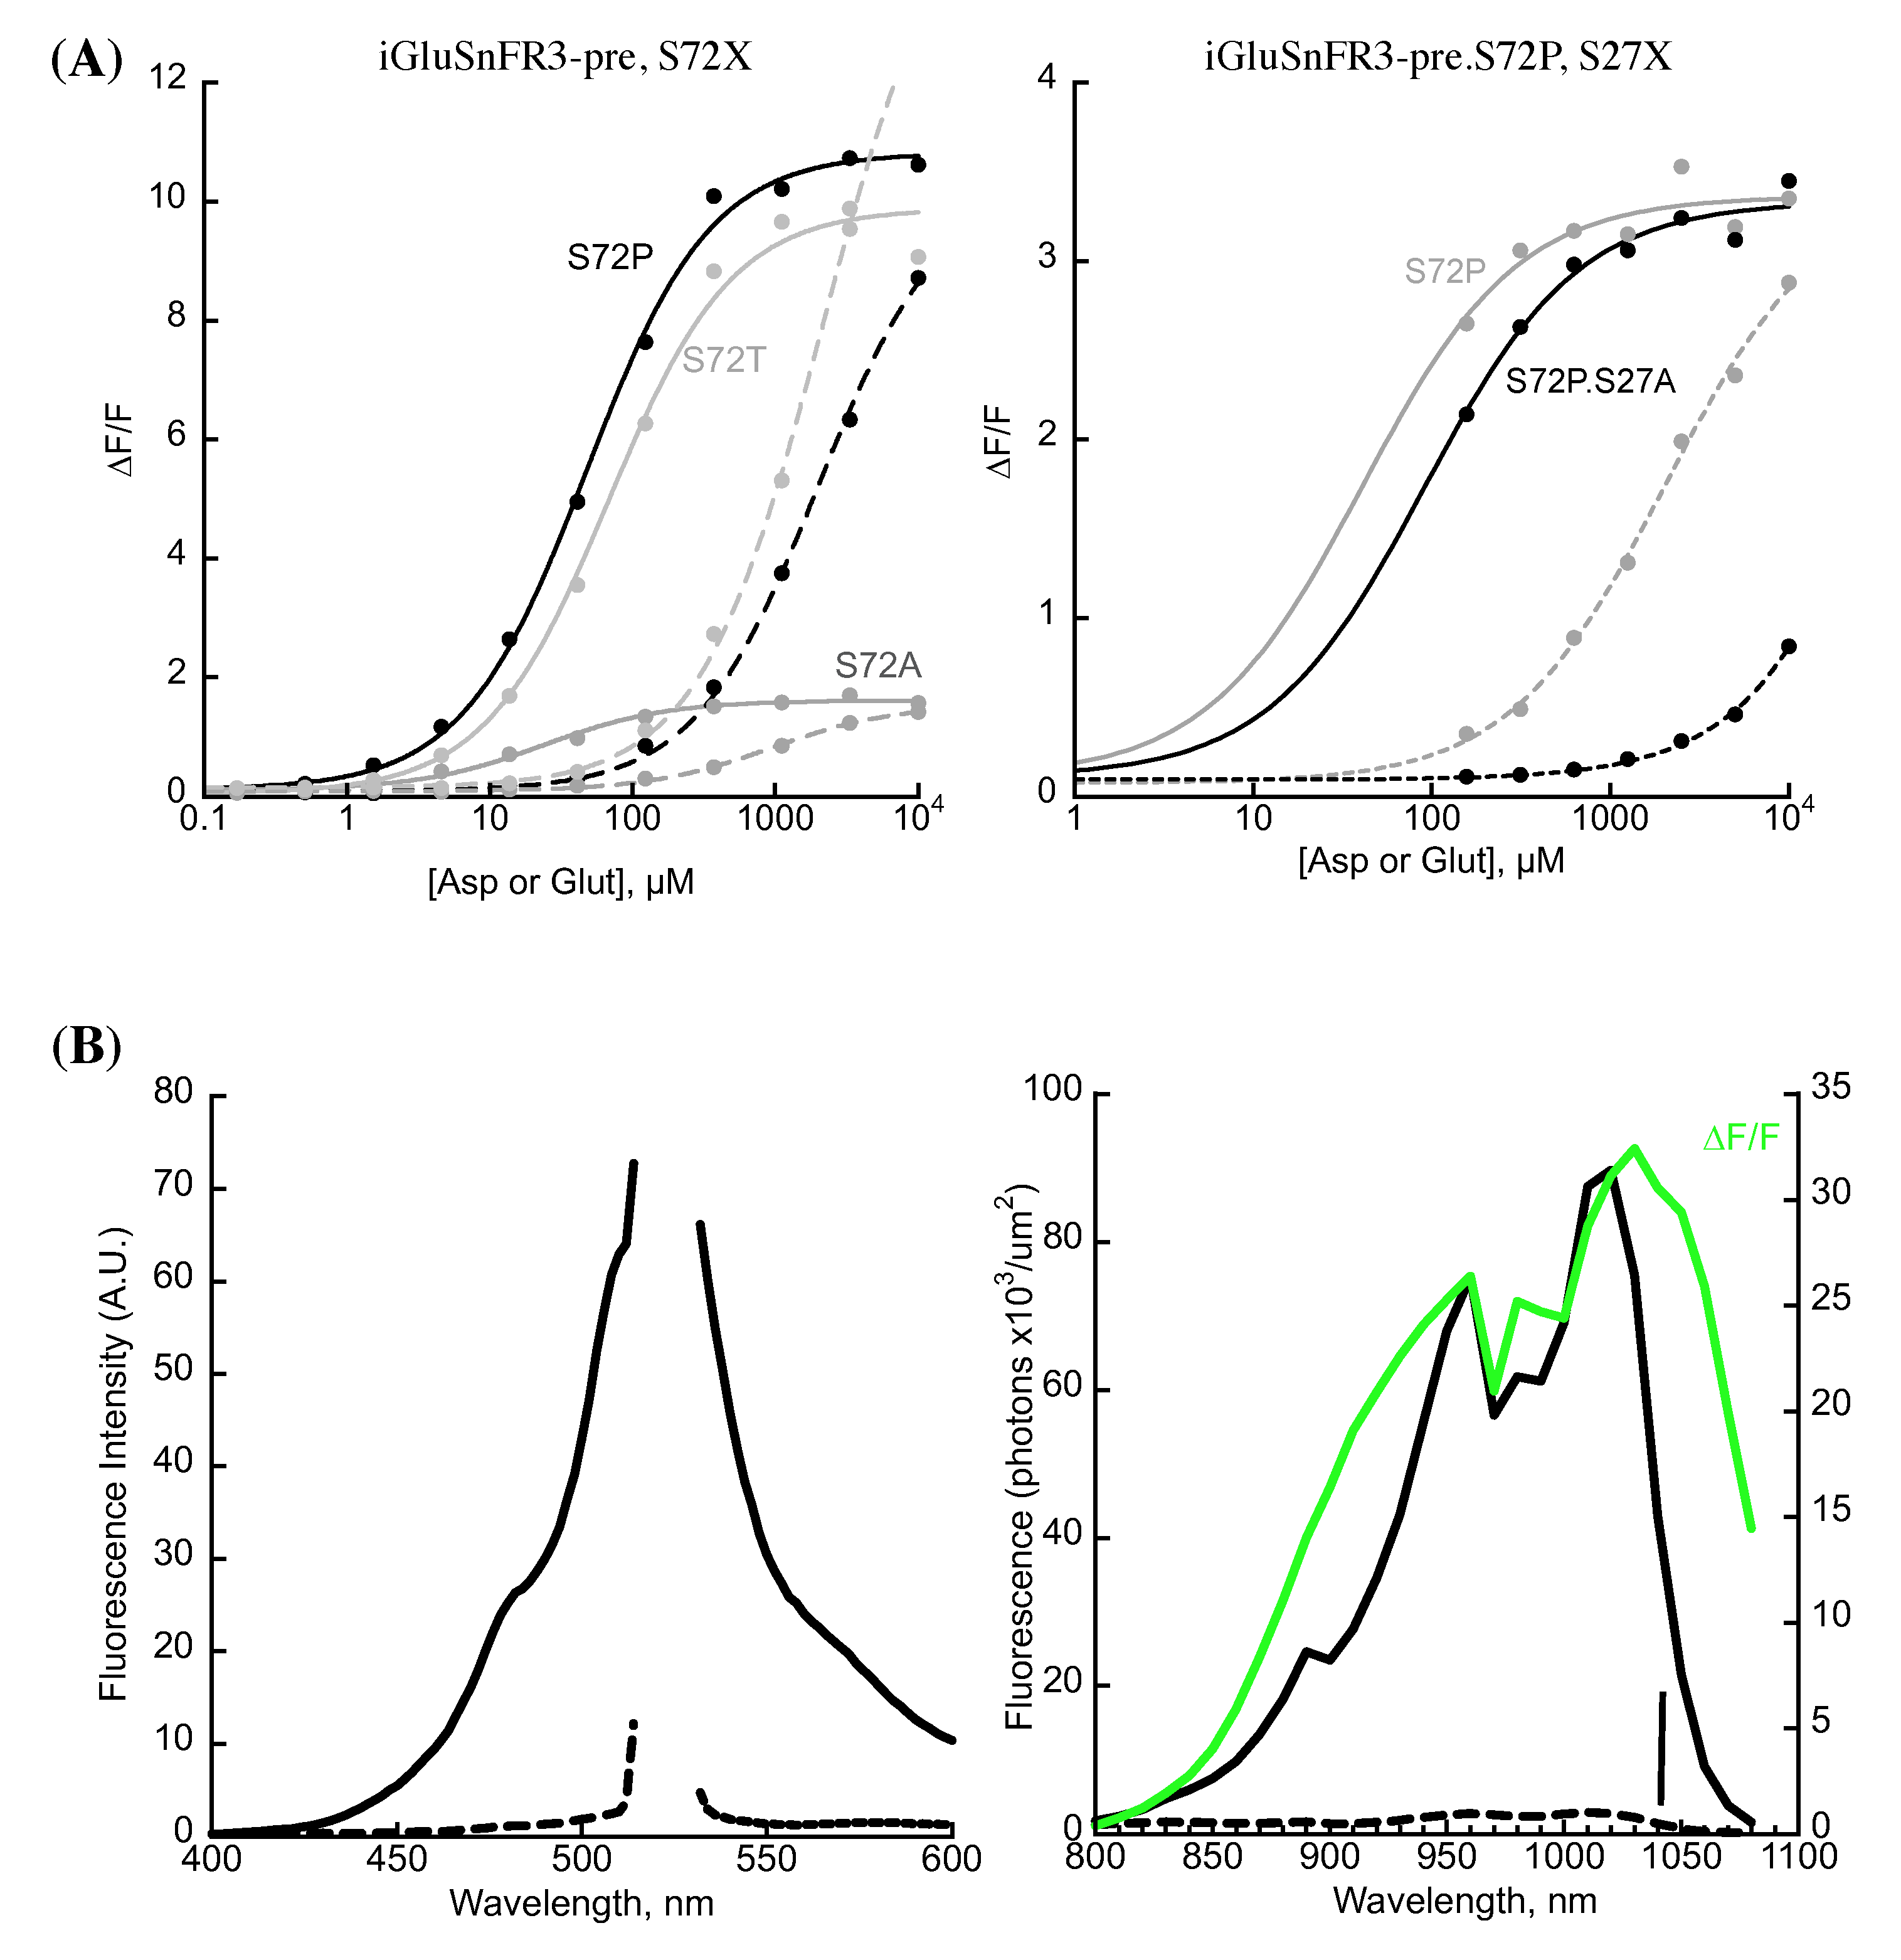
\includegraphics[width=0.7\linewidth]{figures/Fig1S1.pdf}}}\label{figsupp:f1S1}
\figsupp[Decoy, temperature and pH sensitivity.]{
(A) iASPSnFR2.mRuby3 does not appreciably change its green fluorescence in response to other amino acids (alanine, phenylalanine, glycine, histidine (red line), isoleucine, leucine, methionine, proline, glutamine, arginine, serine, threonine, valine, or tryptophan).
Insert with aspartate in black and glutamate/asparagine in grey for comparison.
Ex. 485 nm (20 nm bandpass), Em. 535 nm (20 nm bandpass), 0.2 µM purified protein in PBS.
(B) iASPSnFR2.mRuby3 shows increased red fluorescence at millimolar concentrations of all amino acids, with apparent responses to histidine at 100 µM (red trace).
Ex. 587 nm (20 nm bandpass), Em. 662 nm (20 nm bandpass).
(C) iASPSnFR2.mRuby3 does not respond to other decoys: citrate, lactate, pyruvate, malate, alpha-ketoglutarate, cis-aconitate, succinate, fumarate, or oxaloacetate (orange squares); nor to relevant pharmacological treatments: rotenone (green squares) or metformin.
The small increase in fluorescence from rotenone is likely due to the scattering of a visibly turbid solution; rotenone has very low solubility in water.
Ex. 485 nm (20 nm bandpass), Em. 535 nm (20 nm bandpass).
(D) iASPSnFR2.mRuby3 is not adversely affected by temperature.
Fluorescence as a function of aspartate titration at 23°C (light grey), 30°C (medium grey), and 37°C (black).
Error bars are standard deviation of three technical replicates.
(E) pH sensitivity of iASPSnFR2.mRuby3 (green component).
Ex 485 nm (5 nm bp), Em 515 nm (10 nm bp).
Error bars are standard deviation of 5 technical replicates.
Solid line is with 3 mM aspartate, dashed line is without aspartate.
}{\fbox{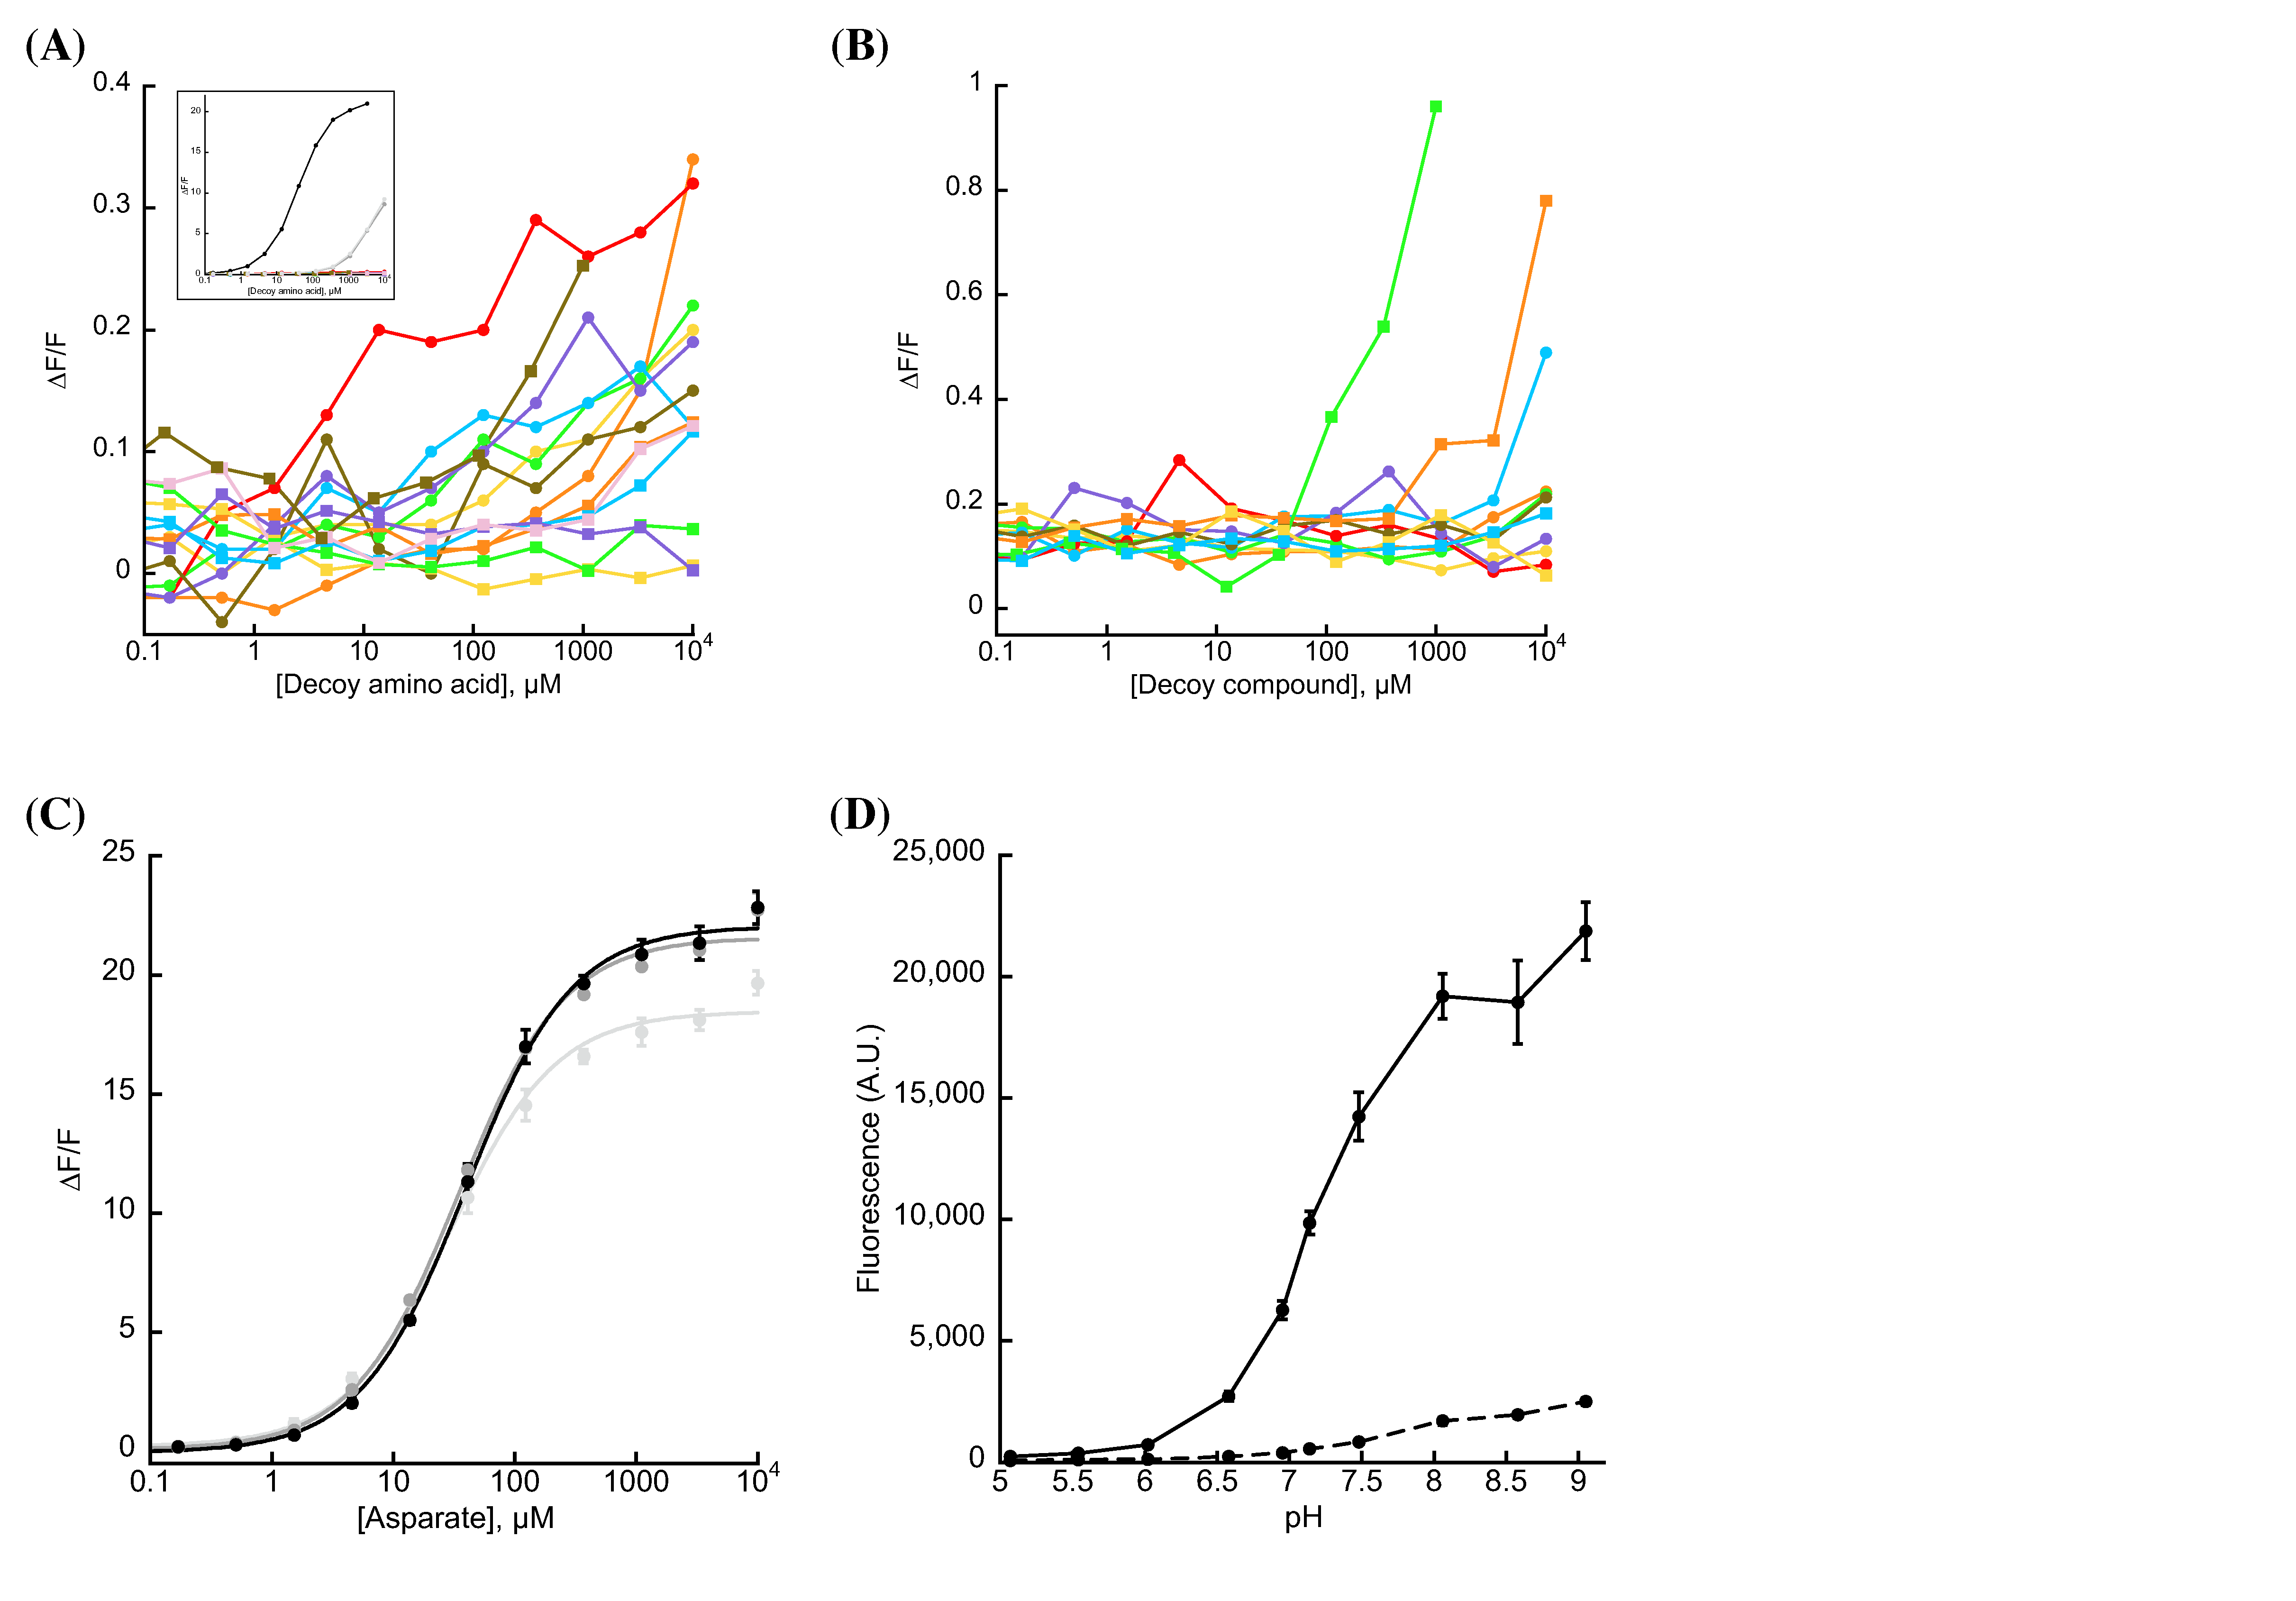
\includegraphics[width=0.98\linewidth]{figures/Fig1S2.pdf}}}\label{figsupp:f1S2}
\end{figure}




\subsection{iASPSnFR2 reveals the temporal dynamics of aspartate limitation}
Having shown that iASPSnFR2.mRuby3 protein can measure the concentration of aspartate \textit{in vitro} through standard equilibrium ligand binding titrations we wanted to test the usefulness of the sensor in cells.
To that end, we generated stable cell lines with constitutive expression of iASPSnFR2.mRuby3 or iASPSnFR2 and nuclear localized RFP, and generated single cell clones from each to yield cell lines with uniform expression of each construct.
In each case, we then normalized GFP sensor signal to RFP signal to control for expression differences within and across cell lines.
We also noted that normalization with nuclear RFP and RFP fusion were highly correlated, enable iASPSnFR2 sensor applications where nuclear RFP labeling is desirable (\FIGSUPP[Fig2]{f2S1}, panel C) e.g. for counting cells at each timepoint.
An important motivation for using a biosensor for tracking aspartate changes is to enable temporal measurements on the same subset of live cells.
To achieve this, we used an Incucyte S3 which performs live cell imaging under native cell line growth conditions.

Aspartate levels are determined in part by its rate of production, which is dependent on the availability of metabolic precursors and the activity of several integrated metabolic processes [overview figure ref].
One such process is the generation of a favorable intracellular NAD+/NADH ratio to drive aspartate precursor synthesis, a process normally maintained through mitochondrial respiration [overview figure ref].
Genetic alterations and pharmacological treatments that disrupt mitochondrial respiration can decrease NAD+/NADH and aspartate levels, both of which can be partially restored by supplementation with alternative electron acceptors, molecules that can restore NAD+/NADH independent of mitochondrial respiration \citep{Sullivan2015-xf, Birsoy2015-pg}.
We thus tested the ability of iASPSnFR2 to quantify changes in intracellular aspartate abundance as a result of treatment with the mitochondrial complex I inhibitor rotenone and the partial rescue of aspartate by additionally supplementing cells with the the alternative electron acceptor pyruvate.
Titrating rotenone in H1299 cells, we observed a dose dependent decrease in sensor fluorescence with increased rotenone, corresponding to the expected decrease in aspartate synthesis capacity (\FIG{Fig2}, panel A).
This observation was extended to different cell lines with different rotenone sensitivities, corroborating the observation of decreased sensor fluorescence upon rotenone treatment and rescue with pyruvate supplementation (\FIGSUPP[Fig2]{f2S1}, panel A, B and D).

We next evaluated the ability of the sensor to measure changes in aspartate without requiring treatment with a mitochondrial inhibitor.
To this aim, we used CRISPR/Cas9 to generate an H1299 cell line with a double knockout (DKO) of the genes glutamic oxalacetic transaminases 1 and 2 (GOT1/2 DKO), which renders cells unable to synthesize aspartate and therefore dependent on aspartate uptake from the media \citep{Garcia-Bermudez2022-qn}.
Using these H1299 GOT1/2 DKO cells, we titrated media aspartate and observed that sensor fluorescence decreased upon aspartate withdrawal and approached a steady-state after approximately 11 hours that corresponded to aspartate availability in the media (\FIG{Fig2}, panel B).
We note that 10 mM media aspartate, a higher concentration than any other amino acid in media, is still unable to rescue sensor signal significantly above aspartate depleted media, confirming previous observations that aspartate has poor cell permeability and often requires 20 mM aspartate or more to robustly contribute to intracellular aspartate pools \citep{Sullivan2018-gz}.


\subsubsection{Metformin has slower kinetics compared to rotenone}
Metformin is a commonly used diabetes treatment that has been shown to act as a mitochondrial complex I inhibitor \citep{Owen2000-ri, El-Mir2000-qm, Andrzejewski2014-wm, Wheaton2014-ka} and can decrease intracellular aspartate levels in a dose responsive way \citep{Gui2016-ca}.
Whereas rotenone is a lipophilic molecule that can cross the cell membrane and act rapidly, metformin is hydrophilic and poorly permeable to most cells, resulting in comparatively delayed kinetics for metformin to decrease mitochondrial respiration in intact cells.
As rotenone and metformin are often used interchangeably as complex I inhibitors, we wondered whether they have an equivalent temporal effect on aspartate or if the delayed effects of metformin on mitochondrial inhibition would similarly delay its effects on aspartate levels.
To test this, we treated cells with two doses each of rotenone and metformin with roughly equivalent aspartate lowering effects and followed the sensor signal over time (\FIG{Fig2}, panel D).
We observed that the aspartate depleting effects of metformin acted more slowly than rotenone, with 30 nM rotenone reaching steady-state after ~20h and 2 mM metformin reaching a similar sensor response after almost 40h.
These data therefore provide orthogonal confirmation of the differential kinetics of these drugs on cell metabolism and highlight the temporal opportunities enabled by measuring aspartate levels by iASPSnFR2.

\begin{figure}[ht!]
\centering
\fbox{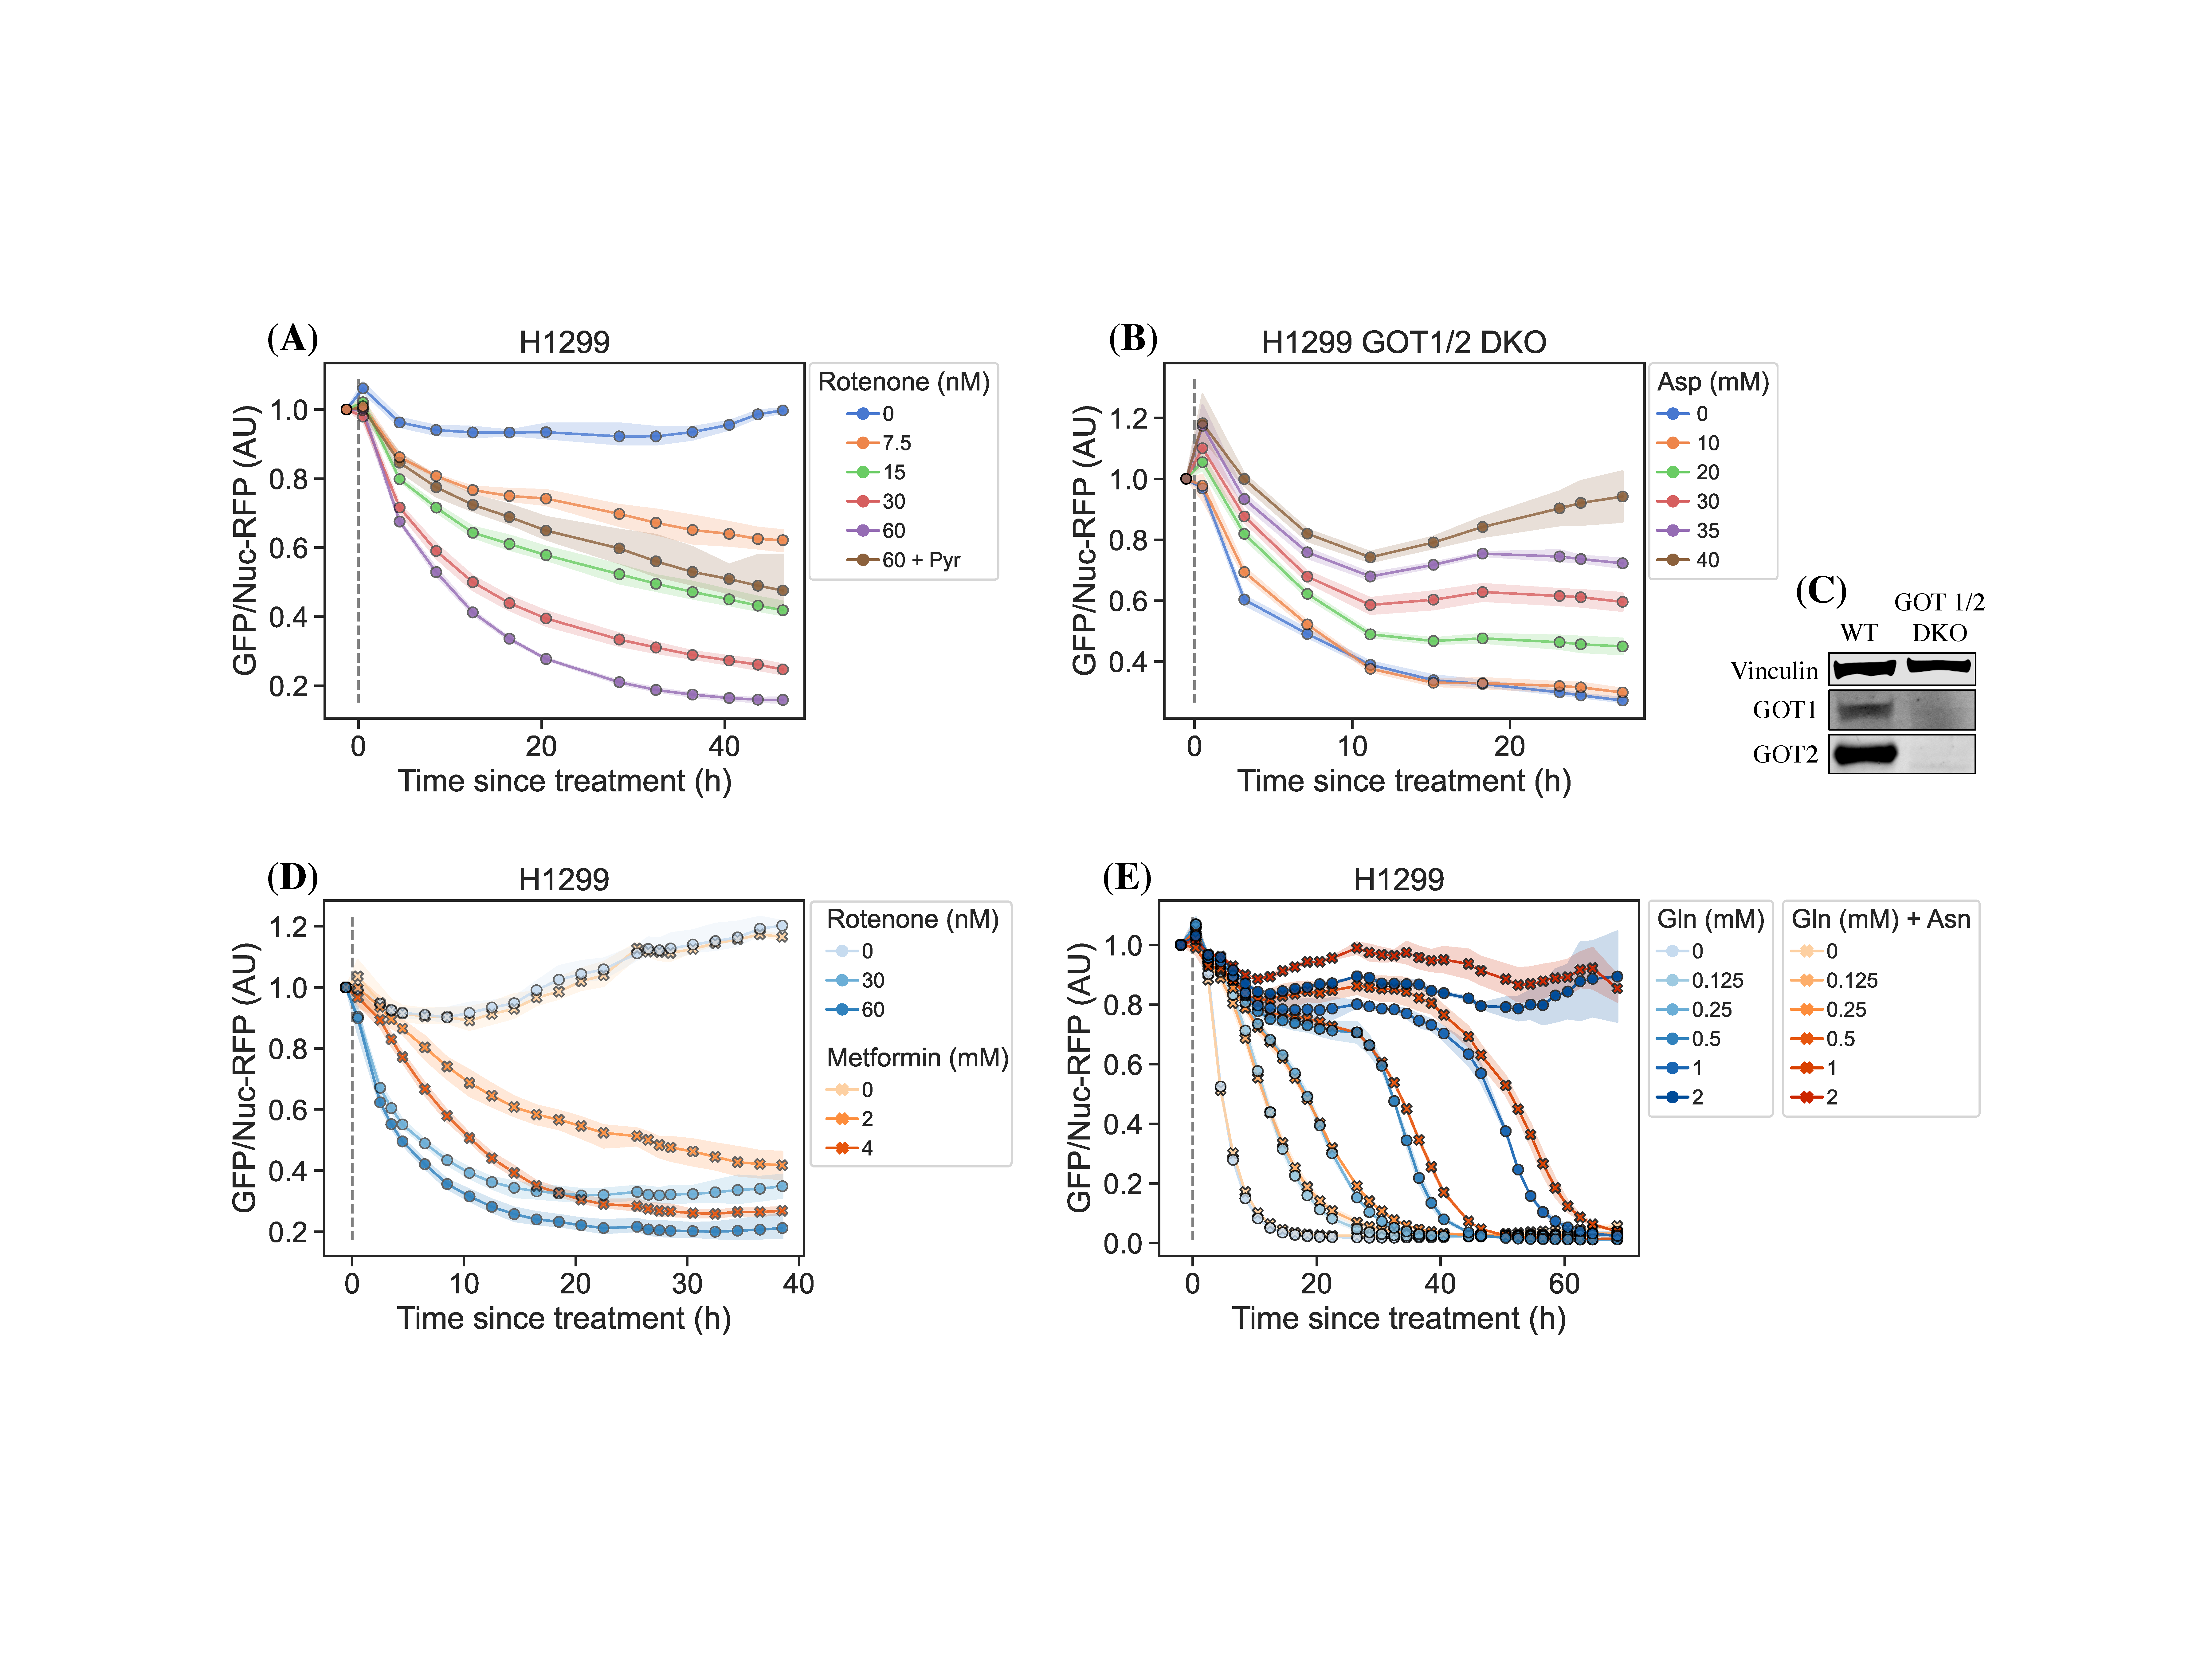
\includegraphics[width=0.95\linewidth]{figures/Fig2.pdf}}
\caption{
iASPSnFR2 resolves temporal aspartate changes in live cells.
RFP normalized iASPSnFR2 signal change over time following various perturbations of live cells.
All experiments shown are normalized to a pre-treatment scan, then treated with the specified drug or amino acid and scanned 30 min following treatment.
Grey dashed lines indicate the time of treatment.
(A) H1299 cells treated with a rotenone titration and rescued by co-treatment with pyruvate.
(B) H1299 GOT1/2 double knockout changed into media with a titration of aspartate.
(C) Western blot verification of H1299 GOT1/2 double knockout.
(D) H1299 cells treated with either rotenone or metformin at the same time to compare inhibitor kinetics.
(E) H1299 cells changed into media with a titration of glutamine with or without 1 mM asparagine.
Markers indicate the average using available well replicates and are superimposed on a bootstrapped 95\% confidence interval colored using the same color code as the markers.
AU, arbitrary unit.
}
\label{fig:Fig2}
\figsupp[Rotenone titration in different cell lines.]{
iASPSnFR2 temporal response after rotenone treatment.
RFP normalized iASPSnFR2 signal change over time following rotenone treatment of live cells.
Related to \FIG{Fig2}, panel A, however; these experiments are not normalized to a pre-treatment scan.
Grey dashed lines indicate the time of treatment and the first scan occurs 30 min after this.
(A) HT1080 cells using nuclear RFP to normalize the iASPSnFR2 signal.
(B) HT1080 cells using an RFP fused to iASPSnFR2 (iASPSnFR2.mRuby3) for normalization.
(C) Comparison between the steady-state signal of (A) and (B) with a linear regression shown as a red dashed line to show that nuclear RFP and RFP fusion normalizations are equivalent.
(D) HEK293t cells using an RFP fused to iASPSnFR2 for normalization.
For plots (A), (B) and (D) markers indicate the average using available well replicates and are superimposed on a bootstrapped 95\% confidence interval colored using the same color code as the markers.
AU, arbitrary unit.
For plot (C) markers indicate the average using available well replicates and errorbars are drawn as +/- the standard deviation of the replicates.
}{\fbox{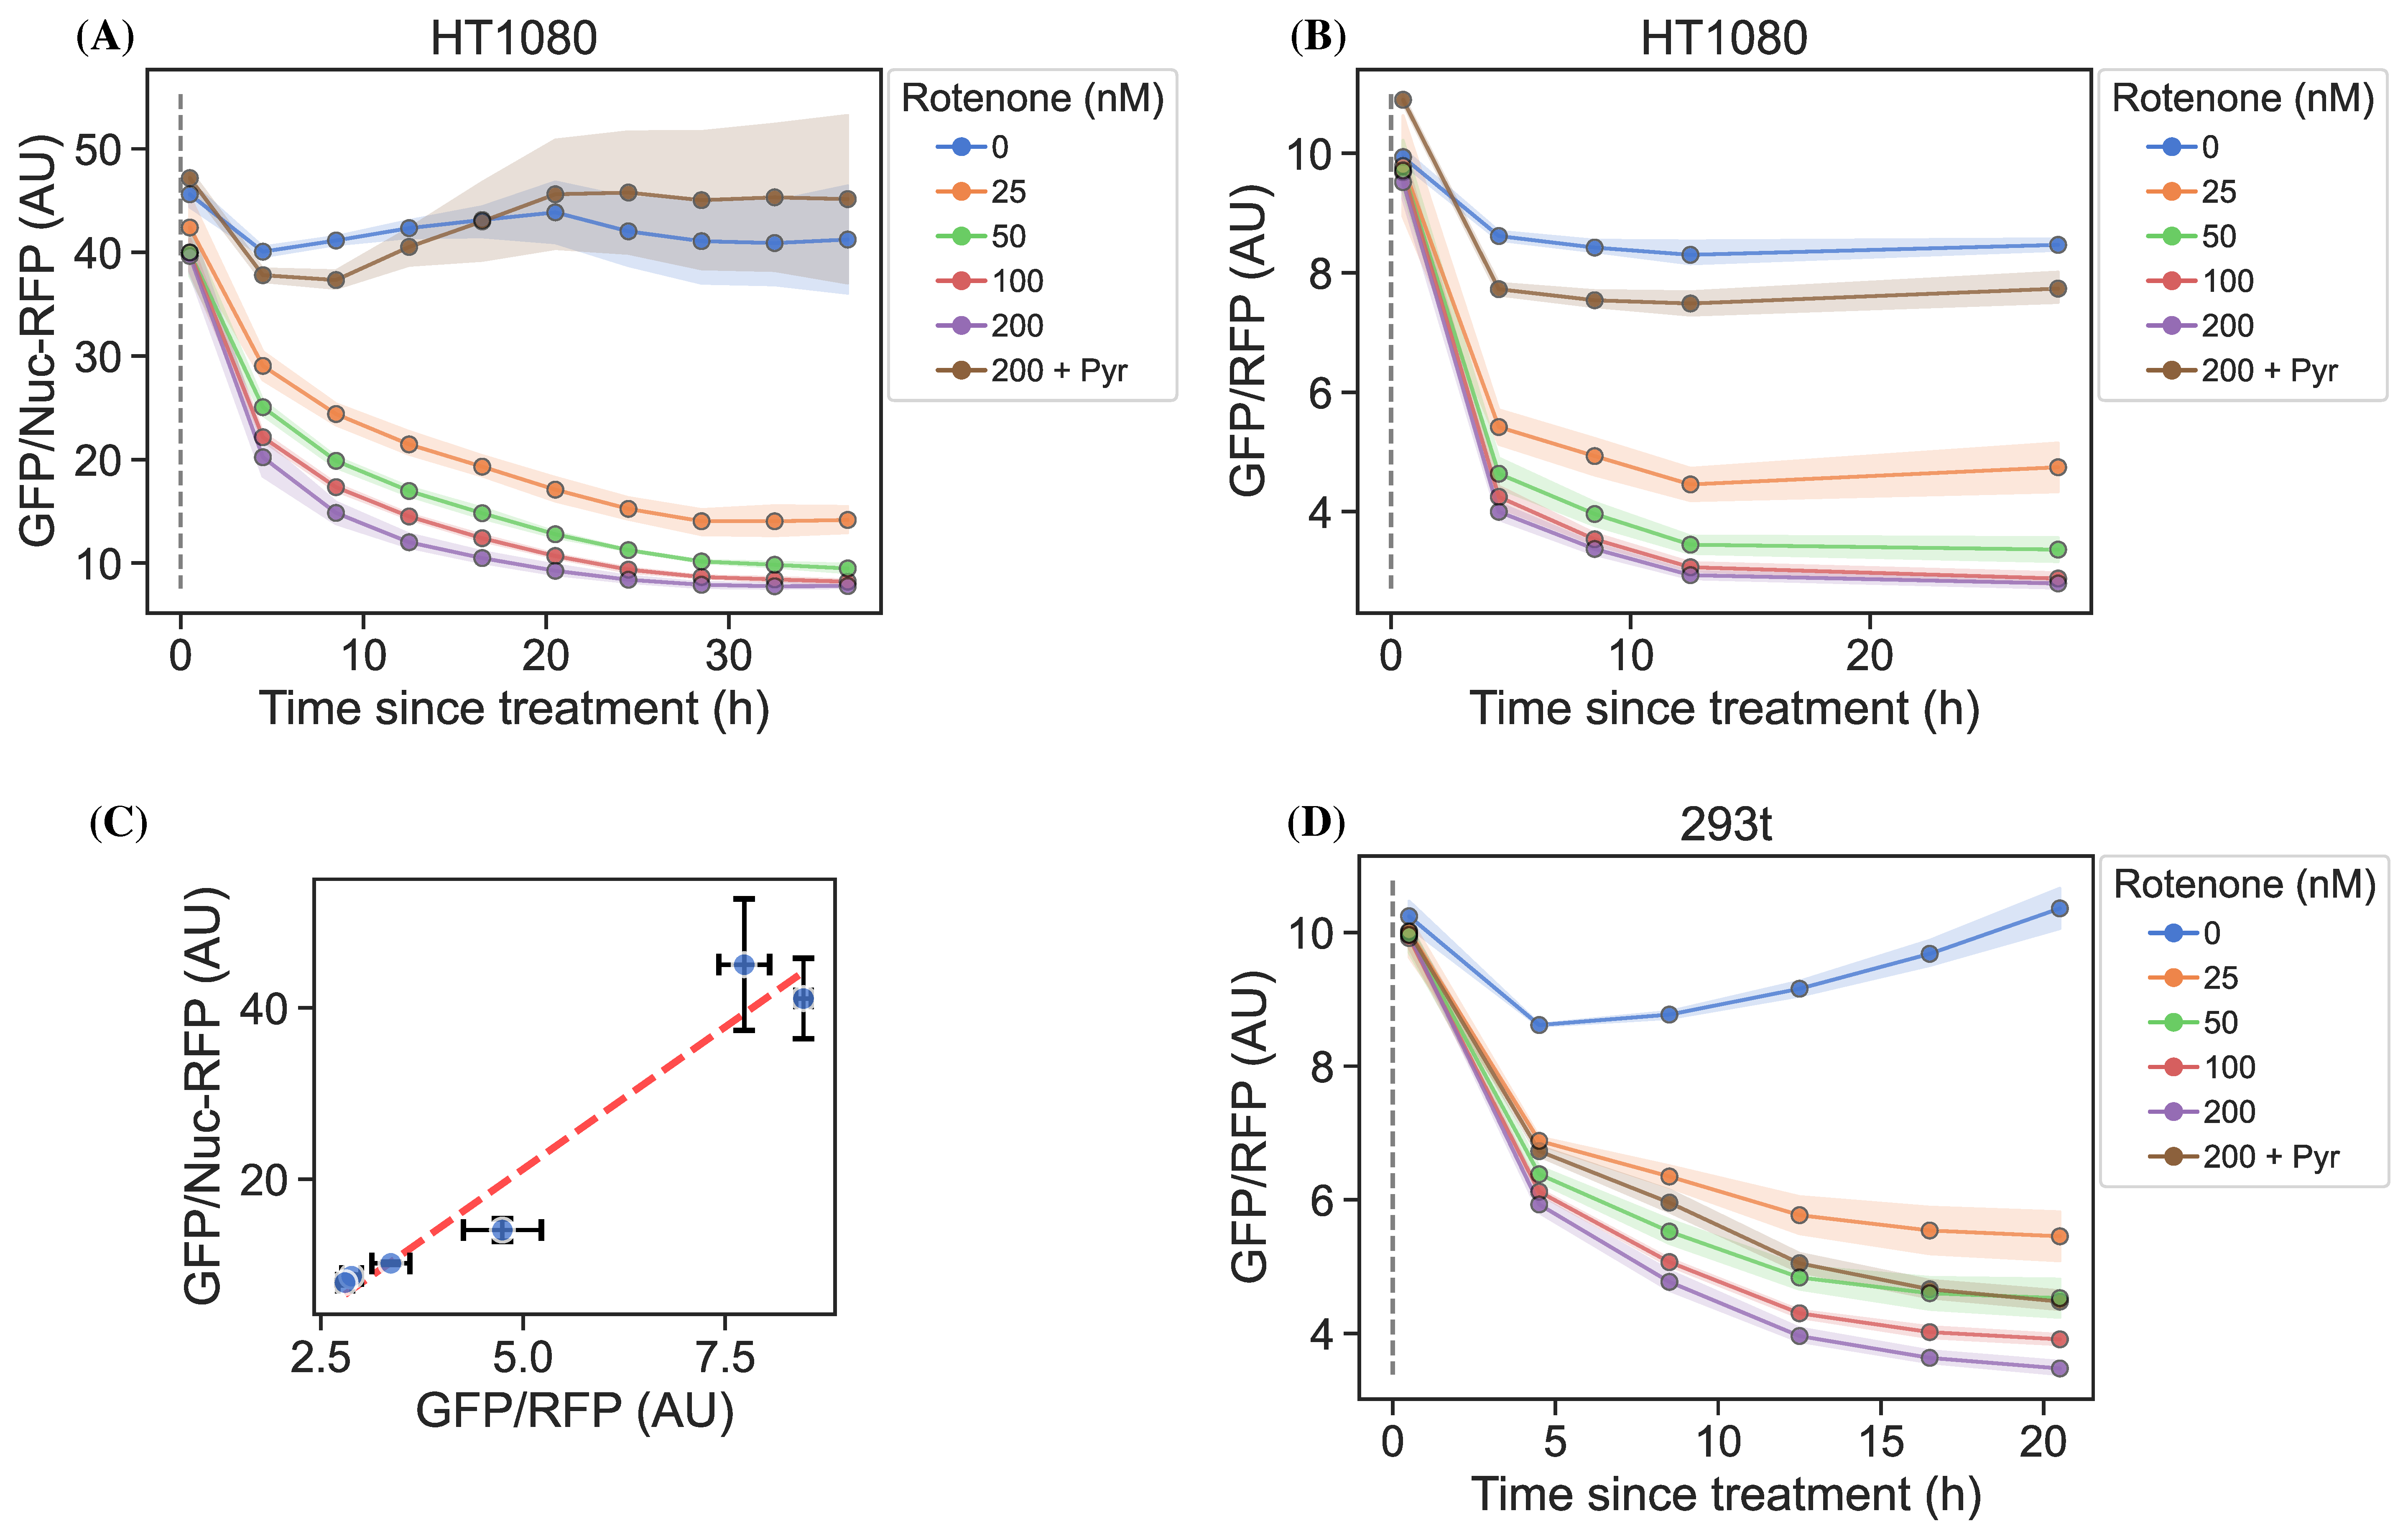
\includegraphics[width=0.98\linewidth]{figures/Fig2S1.pdf}}}\label{figsupp:f2S1}
\figsupp[Narrow range glutamine limitation.]{
Aspartate depletes when glutamine is limiting.
RFP normalized iASPSnFR2 signal change over time following glutamine depletion in H1299 cells.
Identical to \FIG{Fig2}, panel E but with less glutamine concentrations and more well replicates.
AU, arbitrary unit.
}{\fbox{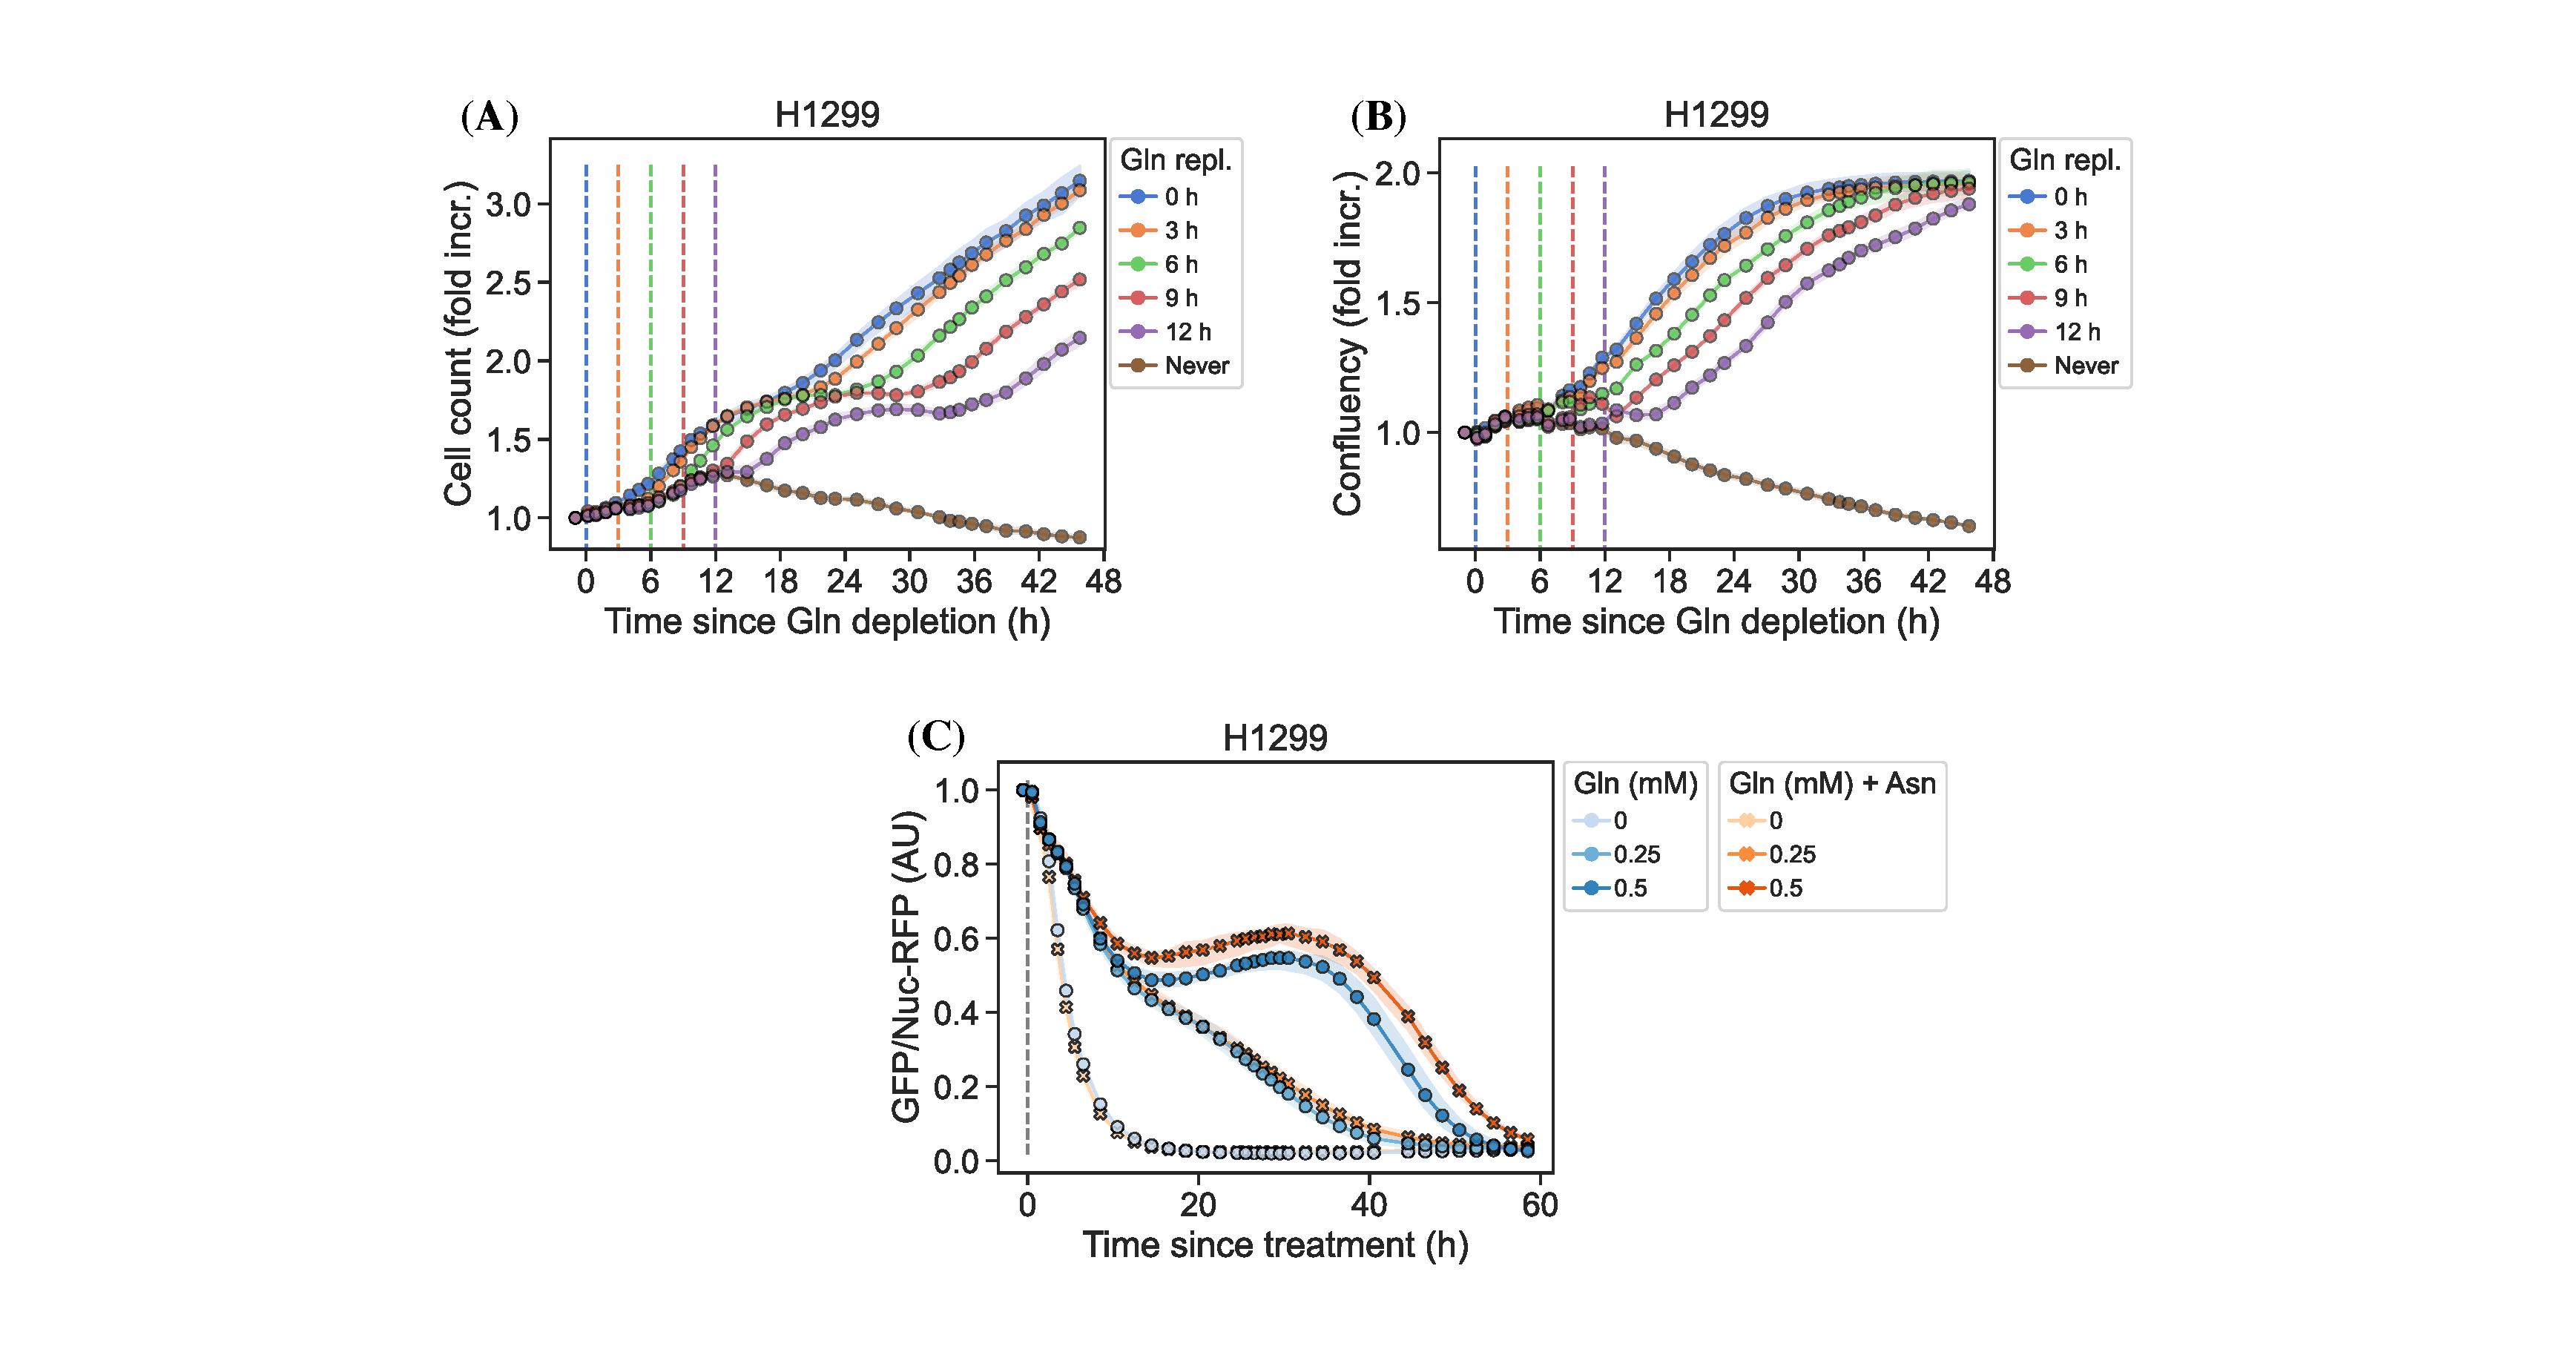
\includegraphics[width=0.65\linewidth]{figures/Fig2S2.pdf}}}\label{figsupp:f2S2}
\end{figure}



\subsubsection{Asparagine salvage diverts glutamine consumption}
In most cancer cell lines, intracellular aspartate is derived primarily from glutamine oxidation, thus making glutamine depletion a potential entry point for affecting aspartate metabolism.
It has previously been reported that asparagine, a product of aspartate metabolism, becomes essential upon glutamine starvation \citep{Pavlova2018-nl, Zhang2014-zz}.
We hypothesize that asparagine becomes essential in these conditions because glutamine starvation decreases synthesis of aspartate, slowing asparagine production, and because asparagine supplementation spares aspartate consumption, allowing it to be redirected into other essential fates.
However, it has been difficult to measure metabolic changes during glutamine limitation because continuous glutamine consumption during the course of the experiment will result in progressive glutamine depletion and further developing metabolic effects.
One solution to this problem is to measure the temporal changes in aspartate levels over the course of glutamine starvation, a possibility enabled by fluorescence based measurements of aspartate using iASPSnFR2.
Indeed, we found that glutamine depletion has a rapid and drastic effect on sensor signal and that this effect was delayed by adding back glutamine (\FIG{Fig2}, panel E).
Aspartate signal did not robustly correlate with the concentration of glutamine in the media in the short term, but instead we found that higher amounts of glutamine in the media delayed the time until aspartate depletion, presumably corresponding to the time at which glutamine is fully depleted and unable to support further aspartate synthesis.
Furthermore, we found that adding 1 mM asparagine also delayed the decrease in sensor signal, suggesting that when asparagine can be salvaged from the media it diverts glutamine consumption that would otherwise be purposed for asparagine synthesis.
We note that, as this data is produced in real-time, the method can be used to dynamically find the optimal sampling times to measure and compare intracellular levels of all the metabolites relevant to glutamine starvation.




\subsection{iASPSnFR2 signal correlates with intracellular aspartate concentration}
It is an important requirement for an aspartate sensor that it reflects the intracellular concentration of aspartate over a biologically relevant range for several cell lines.
Reference points for the intracellular aspartate concentration can be generated using metabolite extraction and LCMS but it is important to note that this technique reports the total amount of aspartate summed across all compartments, which can differ in their aspartate concentration \citep{Chen2016-mf}.
The LCMS derived concentration also does not reflect protein crowding, aspartate binding to enzymes or others factors that would effect the free aspartate concentration.
Nevertheless, LCMS is the standard approach in studying metabolism and has previously been used to correlate aspartate levels with cell proliferation \citep{Gui2016-ca, Hart2023-gp}.
Thus, we titrated mitochondrial inhibitors of complex I (rotenone and metformin) and complex III (antimycin A), followed by pyruvate rescue, in three different cell lines and waited 24 hours until aspartate had reached near steady-state levels before conducting a final measurement of sensor fluorescence, followed by immediate metabolite extraction and quantitative LCMS measurements of aspartate levels using isotopically labeled standards.
We then compared sensor signals to LCMS derived aspartate concentrations and fitted a Hill curve to infer the intracellular aspartate concentrations at half-maximum sensor signal (\FIG{Fig3}).
For all three cell lines, we observe a monotonically increasing relationship between sensor signal and intracellular aspartate concentration covering around two orders of magnitude.
We also observe no relationship between sensor signal and intracellular glutamate levels (\FIGSUPP[Fig3]{f3S1}).
These observations validate the utility of our sensor in a biologically relevant range of aspartate concentrations without interference from glutamate.

Interestingly, the intracellular aspartate concentrations at half-maximum sensor fluorescence is more than 17 fold higher than the aspartate Kd determined by \textit{in vitro} characterization of the sensor.
While the numbers inferred for intracellular aspartate are uncertain point estimates, it is highly unlikely that they are inaccurate to this degree and thus we speculate that the apparent cytosolic aspartate concentration is likely lower than the total aspartate concentration summed across all compartments.
This suggests that binding of aspartate by iASPSnFR2 is in competition with other proteins and highlights another advantage of using biosensor based measurements of metabolite levels in their native environment.




\begin{figure}[ht!]
\centering
\fbox{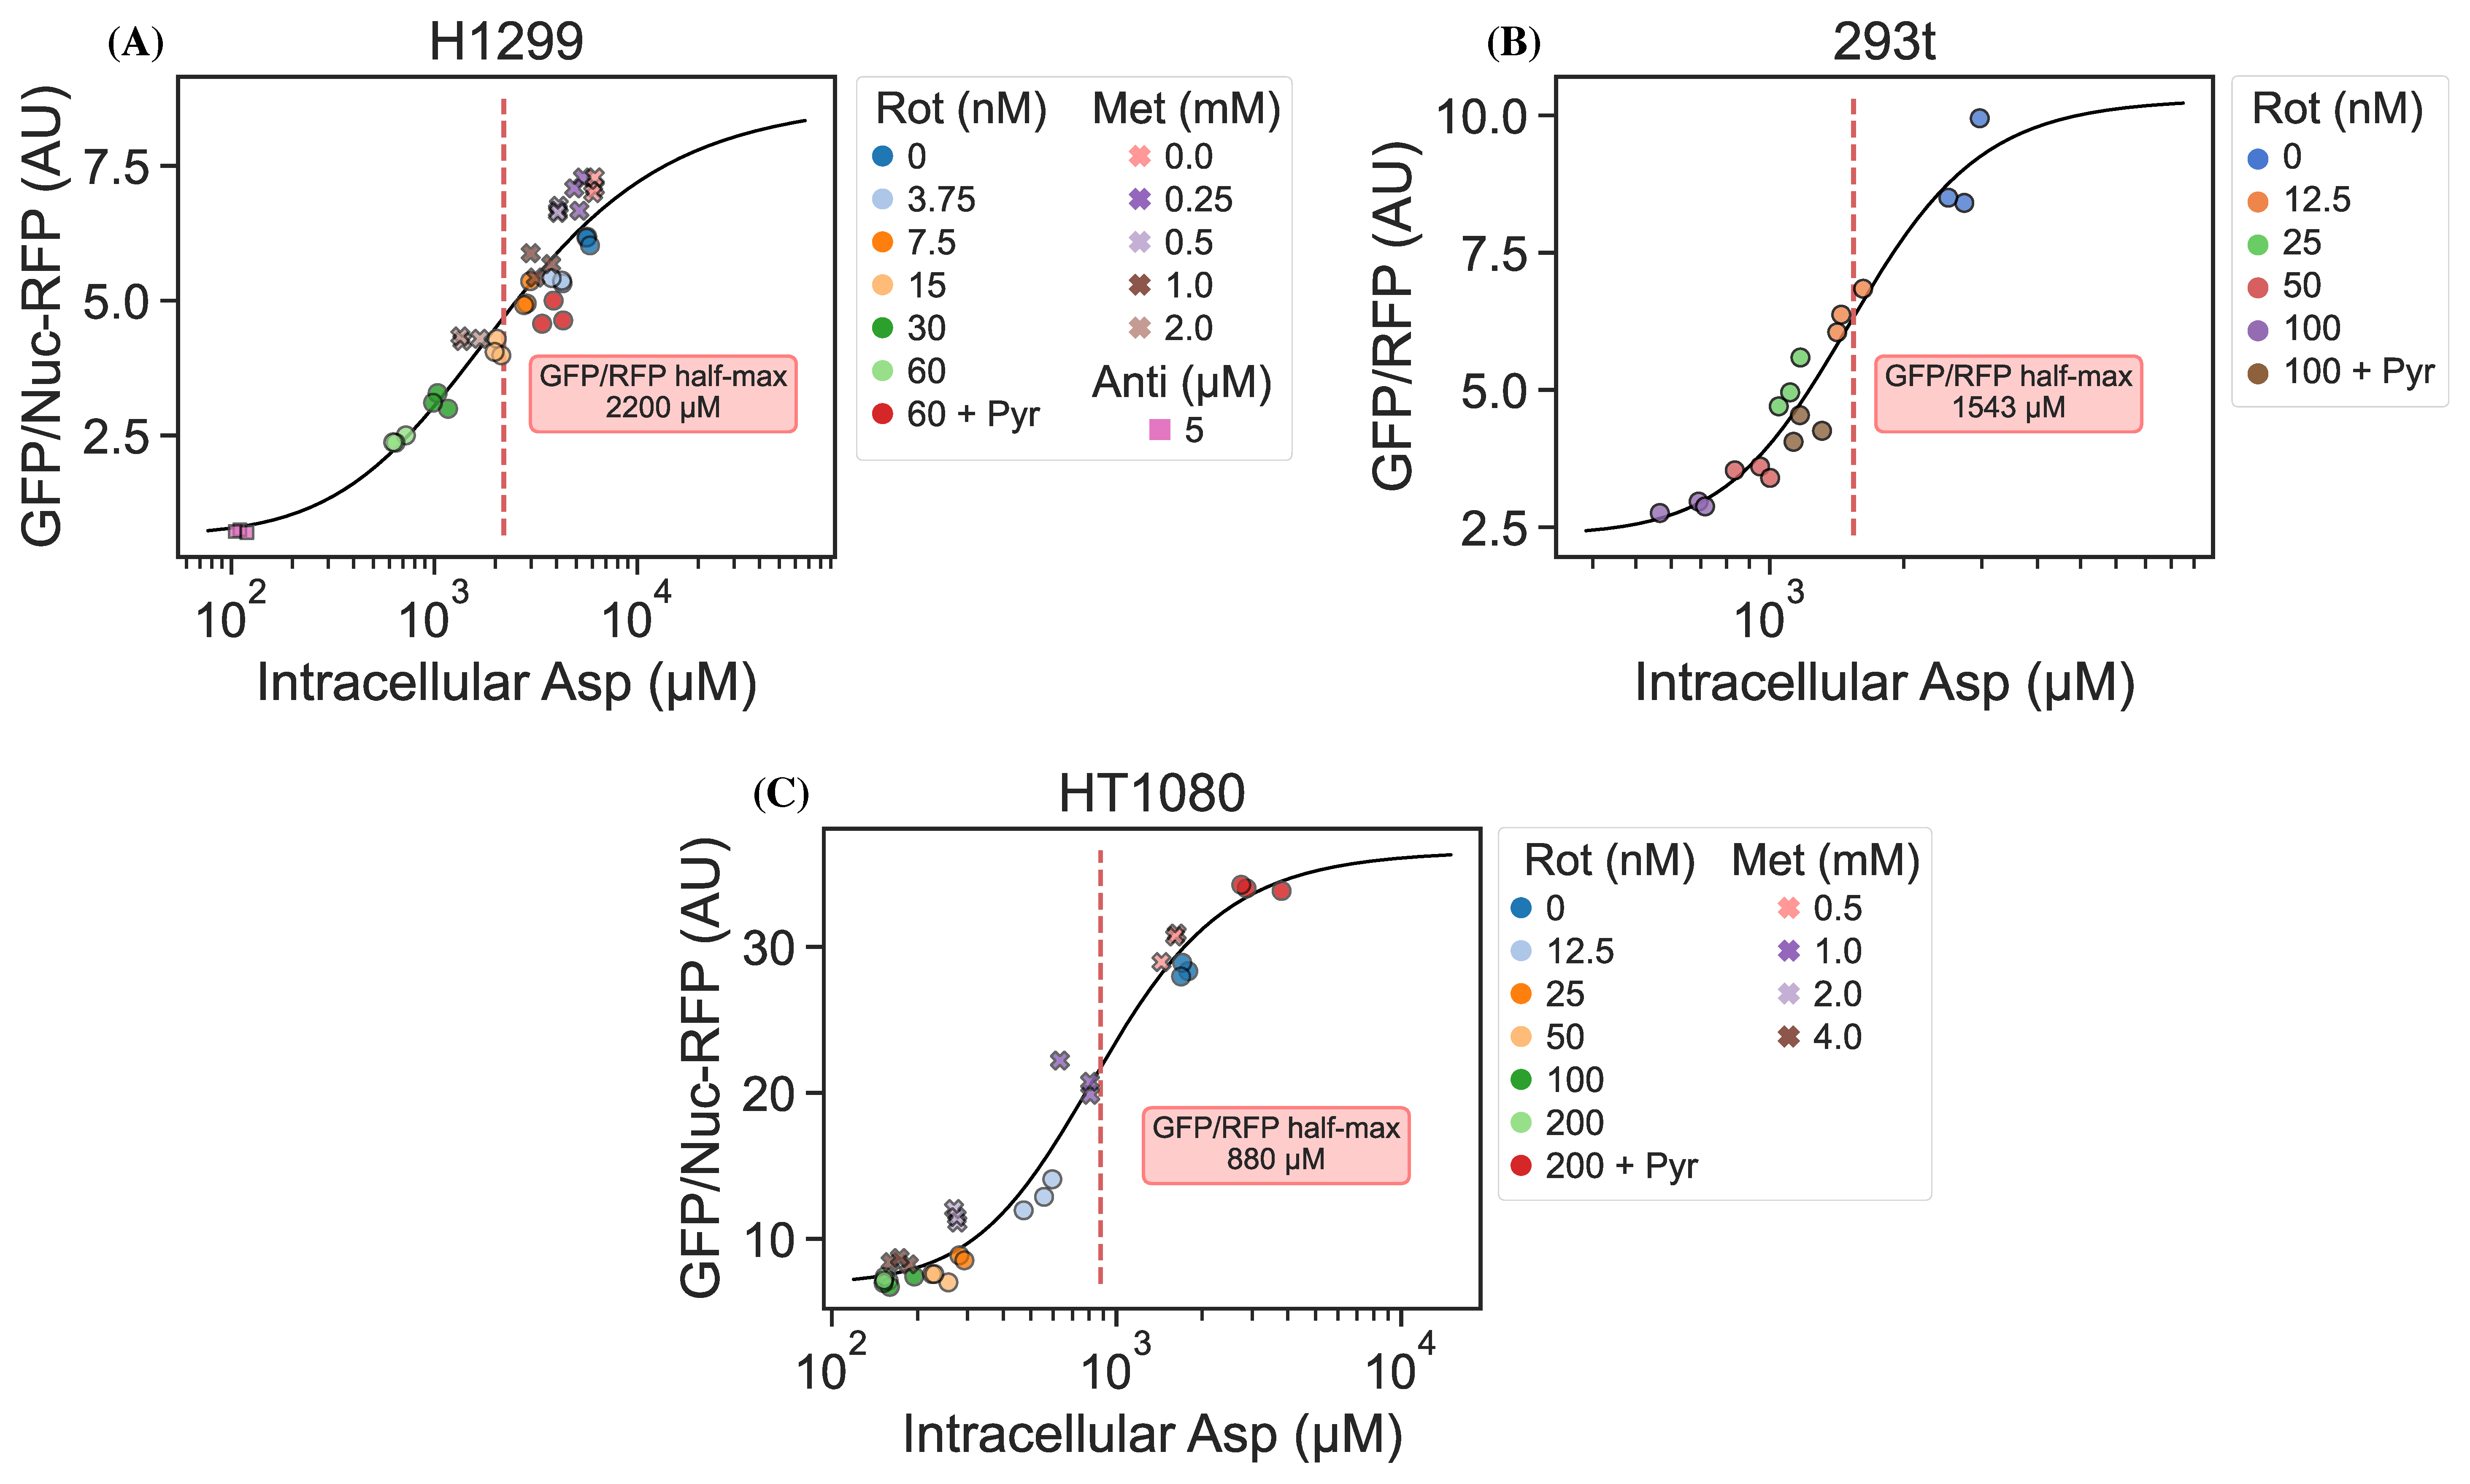
\includegraphics[width=0.98\linewidth]{figures/Fig3.pdf}}
\caption{
iASPSnFR2 signal predicts intracellular aspartate concentration.
RFP normalized iASPSnFR2 signal, following various perturbations to live cells, can predict the LCMS measured intracellular aspartate concentration.
Datapoints are fitted to the Hill equation, shown by the black line, with top and bottom asymptotes, midpoint and slope as free variables.
The intracellular aspartate concentration at the inferred half maximum of RFP normalized iASPSnFR2 signal is reported in the red inserts.
(A) Rotenone titration in HEK293t cells.
(B) Rotenone and metformin titrations in HT1080 cells.
(C) Rotenone, metformin and antimycin A titrations in H1299 cells.
Markers indicate a single well from which both LCMS and iASPSnFR2 data was collected.
Replicate wells have identical color and marker shape.
AU, arbitrary unit.
}
\label{fig:Fig3}
\figsupp[iASPSnFR2 signal does not correlate with glutamate concentration.]{
RFP normalized iASPSnFR2 signal, following various perturbations to live cells, is not correlated with the LCMS measured intracellular glutamate concentration.
Datapoints are fitted to a local linear regression, shown by the black line, otherwise, these plots are identical to those in \FIG{Fig3}.
AU, arbitrary unit.
}{\fbox{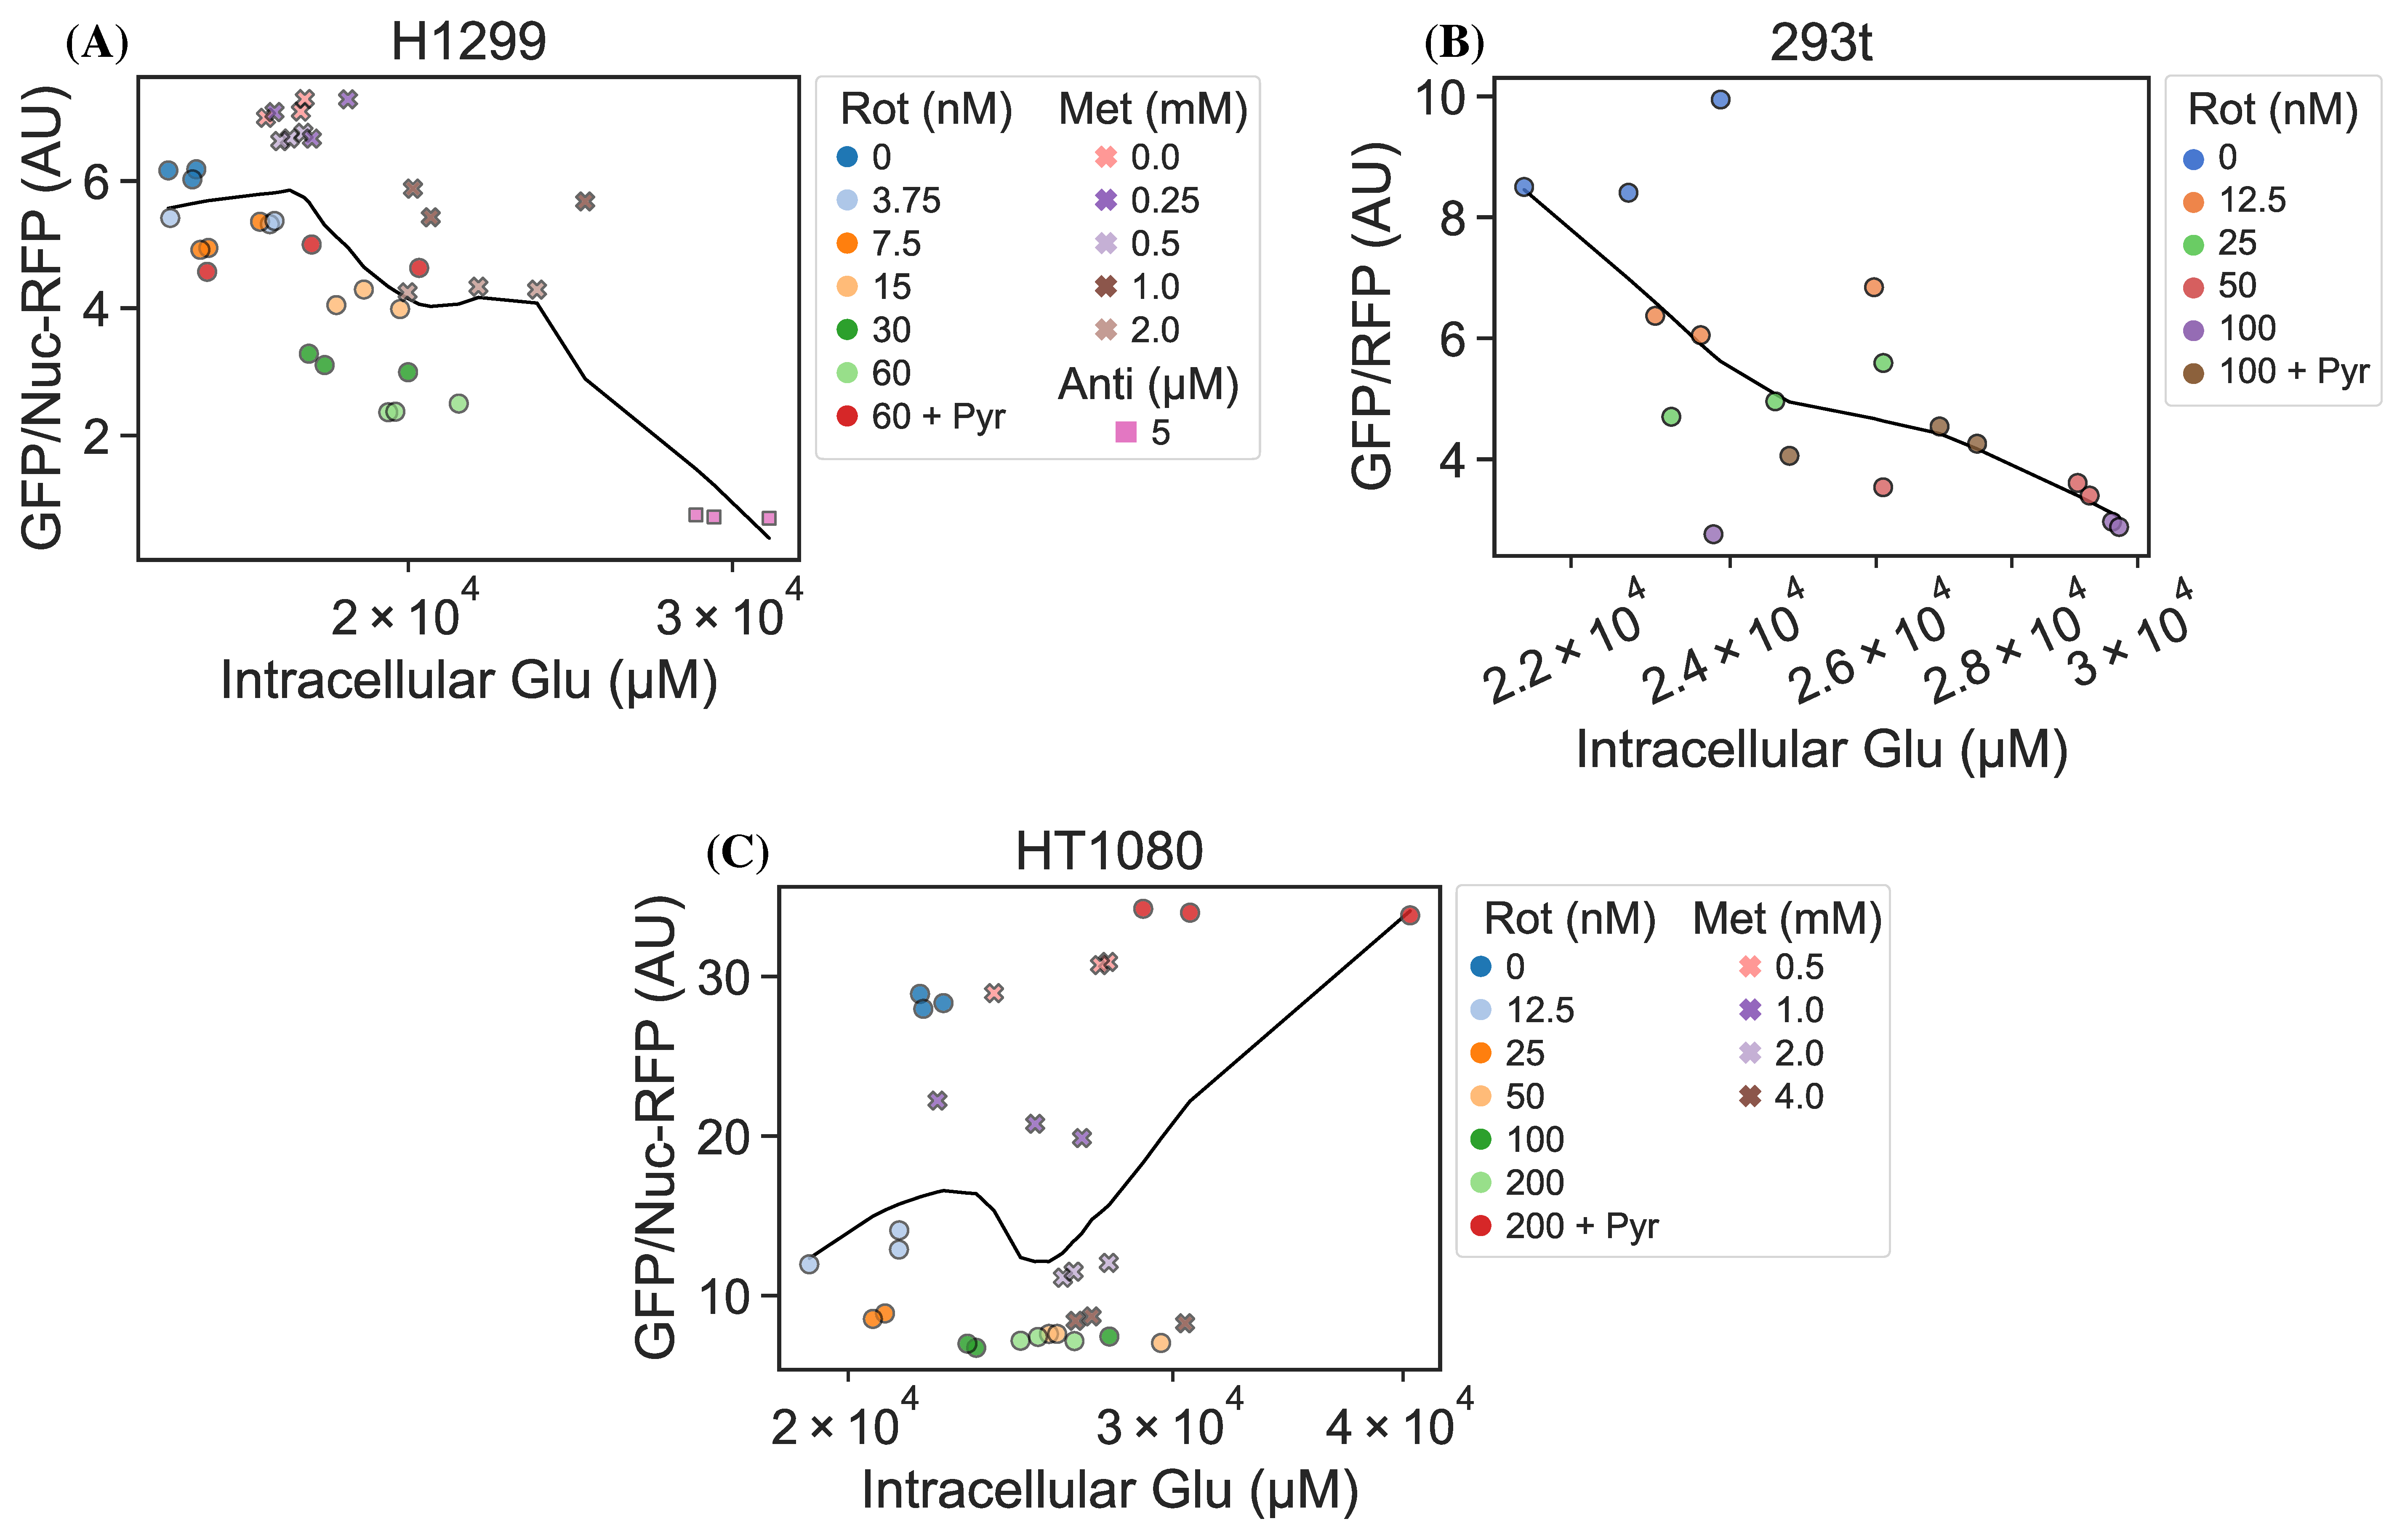
\includegraphics[width=0.98\linewidth]{figures/Fig3S1.pdf}}}\label{figsupp:f3S1}
\end{figure}

%LS - Which cell lines are using which iASPSnFR2 construct? Normalized to nuclear RFP or tagged RFP?
%KD: See y-axis title. It should be consistent throughout. Still think it should be added to figure text?



\section{Discussion}
A biosensor for aspartate is an important step towards improved understanding of aspartate metabolism.
We have shown that our iASPSnFR2 sensor can resolve temporal changes in intracellular aspartate to answer questions that would be impractical using LCMS.
In most studies involving aspartate metabolism, metabolite extraction is performed 6-16 hours after treatment with the implicit assumption that this is enough time to reach metabolic steady-state.
Using our sensor, we have showed that the time to reach steady-state can be much longer and is dependent of the pharmacological treatment.
Future studies seeking to understand the effects of treatments affecting aspartate levels can therefore use real-time measurements using iASPSnFR2 to determine when cells have reached steady-state and then perform metabolite extraction for LCMS.

Recently, a concurrently developed aspartate sensor based on SF-iGluSnFR was reported by another group \citep{Hellweg2023}.
That aspartate sensor started with the S72A mutation (which was shown to preferably bind aspartate over glutamate) but then included 6 additional mutations, apparently making contacts through ever expanding spheres of interaction with the ligand, identified by a combination of targeted screening and deep mutational scanning.
Our design has just 2 mutations in the binding pocket, identified by sequential screening of mutations at two positions (40 different mutants were screened in total).
The starting point of our sensor was a variant along the path to the construction of iGluSnFR3 that was selected for high ∆F/F in response to glutamate in bacterial lysate screens of error-prone PCR libraries.
%LS - This^ sentence sounds like the opposite of what we should be saying. Shouldn't the starting point of this sensor (iASPSnFR2) be a variant along the path to the construction of iGluSnFR3 that was not selected in that study because it lost glutamate specificity and gained aspartate sensitivity? We then built off that version?
Our sensor appears to have a larger signal change both \textit{in vitro }and in live cells and has equal responsiveness at 37°C (the temperature used for all our cell culture experiments) as it is does at 30˚C, although head-to-head comparisons have not been performed.
%KD: We could have tested this more carefully e.g. using SLC1A3
Another difference is that our iASPSnFR2 sensor has a higher affinity for all three relevant ligands (aspartate, asparagine, and glutamate) compared the one reported by \cite{Hellweg2023}; however, we found no discernible effect of treatment with 1 mM asparagine on sensor signal in cell culture experiments and found no correlation between intracellular glutamate concentration and sensor fluorescence across treatment conditions (\FIGSUPP[Fig3]{f3S1}).
Collectively, we conclude that the iASPSnFR2 aspartate sensor reported here has biochemical features that make it ideal for measuring intracellular aspartate levels in live cells.

In summary, we report a novel fluorescence based biosensor that enables dynamic measurements of aspartate.
This tool is free of significant interference from relevant metabolites in physiological intracellular systems and can resolve changes in aspartate from diverse treatment conditions in live cells over time.
This approach to measuring aspartate will also have advantages compared to LCMS based metabolomics including enabling high throughput experiments to identify variables that affect aspartate levels, such as testing the effects of a drug library on cells in multiwell plates or using FACS based selection during genetic screens.
Another potential use for this sensor would be to dissect compartmentalized metabolism, with mitochondria being a critical next target.
Altogether, adoption of iASPSnFR2 to measure aspartate levels will therefore provide novel opportunities to understand this critical node of cell metabolism.



\section{Methods and Materials}

\subsection{Sensor engineering and screening}
The starting template for iASPSnFR2 was a variant along the path of making iGluSnFR3.
Sequence information is in Supp. Figs.
Site saturation mutagenesis at positions S72 and S27 was achieved by the uracil template method \citep{Kunkel1985-ev}.
Mutant libraries (maximum theoretical diversity of 20 each) were transformed into T7 express cells.
Individual colonies were picked into a 96-well plate containing auto-induction media \citep{Studier2005-ki} and shaken at 30˚C for 18-24 hours, then harvested by centrifugation.
Cell pellets were resuspended in PBS and repelleted by centrifgugation 5 times over, then frozen as pellets overnight.
The frozen 96-well plate was thawed by addition of room temperature PBS, agitated by vortexing to resuspend and lyse cells, and then pelleted again.
100 µL clarified lysate was added to each of two black 96-well plates and its fluorescence read.
Aspartate or glutamate was added (final concentration 100 µM) and fluorescence was measured again.
Wells that had a higher ∆F/F for aspartate than glutamate were isolated, titrated with aspartate or glutamate, and sequenced.
After confirming that S72P was the most selective variant for aspartate from a library of S72X, a library of S27X was made in the background of S72P.
The process was repeated, and S72P+S27A was identified as the "best" aspartate sensor.
mRuby3 was subsequently cloned at the C-terminus.

\subsection{Protein expression and purification}
For large scale protein expression and purification, iASPSnFR2.mRuby3 was transformed into T7 express cells, and a single colony was grown in 300 mL auto-induction media \citep{Studier2005-ki} at 30˚C for ~18 hours.
Cells were pelleted by centrifugation at 6000g, resuspended in PBS and 1 M NaCl and frozen.
The resuspended cell pellet was thawed, sonicated on ice (5 sec on, 5 sec off, 10 min), and centirfuged at 6000g to remove cellular debris.
The lysate was further clarified by centrifugation at 350,000g for 1 hour, and then purified by IMAC on a HisTrap FF column, with a 2 mL/min flow rate and elution from 0 to 200 mM imidazole over 120 mL.
Fluorescent fractions were pooled, concentrated by ultrafiltration, and dialyzed in PBS to remove endogenously bound ligands.
Protein concentration was determined by alkaline denaturation, and measurement at A447 (Ext. Coeff. 44,000 M-1 cm-1).

\subsection{Sensor biochemical characterization}
\textit{In vitro} fluorescence measurements were performed on a Tecan Spark plate reading fluorimeter at ~28˚C, with the exception of the controlled temperature measurement, in which a BioTek Cytation 5 was used.
Concentrated iASPSnFR2.mRuby3 protein was diluted to 0.2 µM in PBS for all measurements.
Decoy amino acids and pharmacologues were purchased from Sigma-Aldrich and solvated as 100 mM stocks in PBS, with the exception of rotenone, which was resuspended in DMSO.
Titrations were performed by making serial dilutions (1:2) of the stock compound into PBS, and adding 10 uL of that to 100 uL of 0.2 µM protein solution.
Fluorescence was measured before addition of compound, and ∆F/F was calculated as (F(treatment)-F(initial))/F(initial).

Two-photon cross sections were collected for 1 µM solutions of protein in PBS with or without 10 mM aspartate, excited by pulses from a mode-locked Ti:Sapphire laser (Chameleon Ultra, Coherent, 80 MHz, 140-fs pulse width, 1 mW power at the focus).
Emission was detected by an avalanche photodiode (PDM Series, Micro Photon Devices) with a 550 nm filter (88-nm bandpass).

\subsection{Cell culture}
Cell lines were acquired from ATCC (HEK293T, H1299, HT1080) and tested to be free from mycoplasma (MycoProbe, R\&D Systems).
Cells were maintained in Dulbecco’s Modified Eagle’s Medium (DMEM) (Gibco, 50-003-PB) supplemented with 3.7 g/L sodium bicarbonate (Sigma-Aldrich, S6297), 10\% fetal bovine serum (FBS) (Gibco, 26140079) and 1\% penicillin-streptomycin solution (Sigma-Aldrich, P4333).
Cells were incubated in a humidified incubator at 37°C with 5\% CO2.

\subsection{Generation of nuclear RFP cell lines}
Nuclear expressing cell lines were generated using 1e5 transducing units of EF1A-nuclear RFP lentivirus (Cellomics Technology, PLV-10205-50) by spinfection.
Cells were seeded at 50\% confluency in 6 well dishes and lentivirus was added to fresh media with 8 µg/µL polybrene and added to cells followed by centrifugation (900g, 90 mins, 30°C).
Two days after infection, cells were sorted for high RFP expression using fluorescence-activated cell sorting (FACS).
High RFP cells were then expanded and single-cell cloned by limiting dilution, plating 0.5 cells/well on a 96 well plate.
Plates were then screened for RFP expression and localization using Incucyte S3 (Sartorius) and a suitable clone chosen, expanded, and used for all subsequent experiments.

\subsection{Lentiviral production and stable cell line generation}
iASPSnFR2 and iASPSnFR2-RFP (iASPSnFR2 with a C-termal fusion to mRuby3) were first cloned into entry vector pENTR1A (Fisher, A10462) using NEBuilder HiFI DNA Assembly Cloning Kit (New England BioLabs, E2621).
These donor constructs were then used to transfer their insert into destination vectors: pLX304-CMV-Blast (Addgene, 25890), pLenti-CMV-Hygro (w117-1) (Addgene, 17454 a gift from Eric Campeau \& Paul Kaufman), or pLX304-CAG-Blast using LR Clonase II (Fisher, 11791100).
pLX304-CAG-Blast was generated in house by swapping the CMV promoter region of pLX304-CMV-Blast with a CAG promoter provided on synthetic DNA (Integrated DNA Technologies).
Each plasmid sequence was verified by whole plasmid sequencing (Plasmidsaurus).
Lentivirus was generated by transfection of HEK293T cells with destination vectors plasmid DNA with the packaging plasmids pMDLg/pRRE (Addgene, 12251), pRSV-Rev, (Addgene, 12253) and pMD2.G (Addgene, 12259) and FuGENE transfection reagent (Fisher, PRE2693) in DMEM (Fisher, MT10017CV) without FBS or penicillin-streptomycin.
The supernatant containing lentiviral particles was filtered through a 0.45 µM membrane (Fisher, 9720514) and was supplemented with 8 µg/µL polybrene (Sigma, TR-1003-G) prior to infection.
For infection, cells were seeded at 50\% confluency in 6 well dishes and centrifuged with lentivirus (900g, 90 mins, 30°C).
After 24 hours the media was replaced with fresh media and after 48 hours cells were treated with either 1 µg/mL blasticidin (Fisher, R21001) or 150 µg/mL hygromycin (Sigma-Aldrich, H7772-1G) and maintained in selection media until all uninfected control cells died.
After selection, cells were expanded and single-cell cloned by limiting dilution, plating 0.5 cells/well using 2-3 96 well plates.
These clones were incubated until 10-30\% confluency and screened for high GFP and RFP signal using Incucyte S3 (Sartorius).
The highest expressing monoclonal cells were selected and further expanded on 6 well plates and screened for fluorescence using the Incucyte.
Clones were then expanded and used for subsequent experiments.
Different cell lines received different vector-sensor combinations: HEK293T cells were infected with pLX304-CAG-Blast-iASPSnFR2-RFP, HT1080 with pLenti-CMV-Hygro-iASPSnFR2-RFP and HT1080, H1299 and H1299 GOT1/2 DKO cells expressing nuclear RFP were infected with pLenti-CMV-Hygro-iASPSnFR2.

\subsection{Generation of GOT1/2 double knockout (DKO) cells}
Protocol and guide RNA generation was identical to that described in \cite{Hart2023-gp}.
Briefly, three chemically synthesized 2'-O-methyl 3’phosphorothioate-modified single guide RNA (sgRNA) sequences targeting GOT1 and GOT2 were purchased (Synthego), sgRNA sequences are shown in the table below (\TABLE{guides}).
A pool of six sgRNAs for GOT1 and GOT2 were resuspended in nuclease-free water, combined with SF buffer (Lonza, V4XC-2032), and sNLS-spCas9 (Aldevron, 9212).
200,0000 H1299 cells were resuspended in the resulting solution containing ribonucleoprotein complexes (RNPs) and electroporated using a 4D-Nucleofector (Amaxa, Lonza).
Nucleofected cells were then expanded and single-cell cloned by limiting dilution by plating 0.5 cells/well in a 96 well plate.
Gene knockout was confirmed using western blots.

\begin{table}[h!]
\caption{\label{tab:guides}CRISPR guides.}
\begin{tabular}{|l|l|}
\hline
Gene & sgRNA   sequence (5’-3’) \\
\hline
GOT1 & \begin{tabular}[c]{@{}l@{}}\texttt{CAGUCAUCCGUGCGAUAUGC}\\\texttt{GCACGGAUGACUGCCAUCCC}\\\texttt{CGAUCUUCUCCAUCUGGGAA}\end{tabular} \\
\hline
GOT2 & \begin{tabular}[c]{@{}l@{}}\texttt{UUUCUCAUUUCAGCUCCUGG}\\\texttt{CGGACGCUAGGCAGAACGUA}\\\texttt{UCCUUCCACUGUUCCGGACG}\end{tabular} \\
\hline
\end{tabular}
\end{table}


\subsection{Intracellular iASPSnFR2 measurements}
Experiments were conducted in DMEM without pyruvate (Corning 50-013-PB) supplemented with 3.7 g/L sodium bicarbonate 10\% dialyzed fetal bovine serum (FBS) (Sigma-Aldrich, F0392) and 1\% penicillin-streptomycin solution.
To start an experiment, cells were trypsinized (Corning, 25051CI), resuspended in media, counted using a coulter counter (Beckman Coulter, Multisizer 4) and seeded onto 24-well dishes (Nunc, 142475) with an initial seeding density of 50,000, 70,000, 70,000 or 150,000 cells/well for H1299, H1299 GOT1/2 DKO, HT1080 and HEK293T, respectively.
After 24h (H1299, HT1080, HEK293T) or 48h (H1299 GOT1/2 DKO) incubation treatment was added and plates moved into an Incucyte S3 (Sartorius) live cell imaging platform inside a humidified incubator at 37°C with 5\% CO2.
Rotenone (Sigma-Aldrich, R8875), metformin (Sigma-Aldrich, D150959) and antimycin A (Sigma-Aldrich, A8674) treatments were spiked-in as 20x solutions in water and the 2 mM pyruvate (Sigma-Aldrich, P8574) was added as 1000x stock.
For treatments with varying media aspartate (Sigma-Aldrich, A7219) or glutamine (Sigma-Aldrich, G5792), wells were thrice washed and filled with media deplete of the given amino acid, then it was added as a spike-in at the specified concentration as 20x solutions in water.
For plates receiving asparagine (Sigma-Aldrich, A7094), this was added to 1 mM from as 20x solution in water, with vehicle wells receiving water.
Live cell imaging was performed on the Incucyte S3 using the GFP and RFP channels with default exposure times.
Images were processed using the associated Incucyte software to subtract background, define areas of cell confluence and GFP/RFP signal and extract the sum of the fluorescence signal in these areas.
The data for the GFP signal, RFP signal, GFP/RFP ratio and confluence for each well at each timepoint was exported and used for further data processing using Python code.
The iASPSnFR2 signal (GFP channel) was normalized to an RFP signal, either as a stably expressed nuclear localized RFP (Nuc-RFP) or mRuby3 C-term fusion to iASPSnFR2.
For temporal measurements the first scan was made 30 min after treatment with subsequent scans indicated on relevant plots.
For some experiments a pre-treatment scan was made shortly prior to treatment to normalize the data to this point.
For comparisons of near steady-state measurements of GFP/RFP versus mass spectrometry based metabolite measurements, a single scan was made 24h after treatment, the plate was then quickly moved to ice and metabolite extraction performed (see below).
Another plate was processed in parallel for cell volume determination using a coulter counter and averaging across three replicate wells.
The normalized iASPSnFR2 signal as a function of intracellular aspartate concentration (c) was fitted by a baseline shifted Hill curve:

$$
f(c) = t + \frac{b - t}{1 + (c/m)^s}
$$

With $t$, $b$ being the top and bottom of the curve, respectively, describing the upper and lower asymptotes of normalized iASPSnFR2 signal.
The curve slope is described by $s$, also known as Hill coefficient, and the midpoint ($m$) describes the intracellular aspartate concentration at half maximum iASPSnFR2 signal.
The curve parameters were fitted to the data using the Broyden–Fletcher–Goldfarb–Shanno (BFGS) algorithm with an upper bound constraint on the top of the curve of 1.2 times the maximum observed normalized iASPSnFR2 signal in any of the conditions on the same plot.
Notice, that this curve is not suppose to represent a mechanistic model of the binding kinetics, rather the purpose is to infer a reasonable estimate of the intracellular aspartate concentration at half maximum iASPSnFR2 signal.

\subsection{Metabolite extraction}
For polar metabolite extraction, a plate was move to ice and the media was thoroughly aspirated.
For H1299 and HT1080 cells, wells were washed once with cold saline (Fisher, 23293184).
For HEK293T cells, washing was omitted due to weak cell adherence.
Then, 1 mL 80\% HPLC grade methanol in HPLC grade water was added, cells were scraped with the back of a P1000 pipet tip and transferred to Eppendorf tubes.
Tubes were centrifuged (17,000g, 15 mins, 4°C) and 800 µL of the supernatant containing polar metabolites was transferred to a new centrifuge tube and placed in a centrivap until dry.

\subsection{Intracellular amino acid concentration measurements}
Dried samples were reconstituted with 40 µL 80\% HPLC grade methanol containing 5 µM U-13C, U-15N labelled canonical amino acid mix (Cambridge Isotope Laboratories, MSK-CAA-1) and transferred to vials for measurement by LCMS.
The peak area for each amino acid was divided by its labelled standard to derive the response ratio.
The response ratio was then mapped to a calibration curve to infer the amino acid concentration and finally the intracellular concentration was calculated by correcting for each step introducing a dilution, including the use of the total cell volume.
To make the calibration curves a non-labelled amino acid mixture was made from an analytical amino acid standard without glutamine and asparagine (Sigma-Aldrich, A9906-1ML) and added glutamine (Sigma-Aldrich, 76523-100MG) and asparagine (Sigma-Aldrich, 51363-100MG) to match the concentration of the other amino acids.
Using this mix, three replicates of a 12 point 2-fold dilution series was made with a max concentration of 500 µM and a volume per dilution of 40 µL.
These were placed in a centrivap until dry and reconstituted with 40 µL 80\% HPLC grade methanol containing 5 µM U-13C, U-15N labelled canonical amino acid mix (Cambridge Isotope Laboratories, MSK-CAA-1) and transferred to vials for measurement by LCMS.
The peak area for each amino acid was divided by its labelled standard to derive the response ratio, then the best fitting calibration curves for each amino acid were chosen among either linear, power or a second-degree polynomial.
Each calibration curve was manually inspected for proper fit and measurements below or above the concentration range of the dilution series were discarded.

\subsection{Liquid Chromatography-Mass Spectrometry (LCMS)}
Metabolite quantitation was performed using a Q Exactive HF-X Hybrid Quadrupole-Orbitrap Mass Spectrometer equipped with an Ion Max API source and H-ESI II probe, coupled to a Vanquish Flex Binary UHPLC system (Thermo Scientific).
Mass calibrations were completed at a minimum of every 5 days in both the positive and negative polarity modes using LTQ Velos ESI Calibration Solution (Pierce).
Polar Samples were chromatographically separated by injecting a sample volume of 1 μL into a SeQuant ZIC-pHILIC Polymeric column (2.1 x 150 mm 5 mM, EMD Millipore).
The flow rate was set to 150 mL/min, autosampler temperature set to 10 °C, and column temperature set to 30 °C.
Mobile Phase A consisted of 20 mM ammonium carbonate and 0.1 \% (v/v) ammonium hydroxide, and Mobile Phase B consisted of 100\% acetonitrile.
The sample was gradient eluted (\%B) from the column as follows: 0-20 min.: linear gradient from 85\% to 20\% B; 20-24 min.: hold at 20\% B; 24-24.5 min.: linear gradient from 20\% to 85\% B; 24.5 min.-end: hold at 85\% B until equilibrated with ten column volumes.
Mobile Phase was directed into the ion source with the following parameters: sheath gas = 45, auxiliary gas = 15, sweep gas = 2, spray voltage = 2.9 kV in the negative mode or 3.5 kV in the positive mode, capillary temperature = 300 °C, RF level = 40 \%, auxiliary gas heater temperature = 325°C.
Mass detection was conducted with a resolution of 240,000 in full scan mode, with an AGC target of 3,000,000 and maximum injection time of 250 msec.
Metabolites were detected over a mass range of 70-850 m/z.
Quantitation of all metabolites was performed using Tracefinder 4.1 (Thermo Scientific) referencing an in-house metabolite standards library using ≤ 5 ppm mass error.

\subsection{Data analysis and plotting}
All data processing, curve fitting, plotting and statistics for experiments involving iASPSnFR2 expressed in cell lines was made using Python code and data available on Github:
\url{www.github.com/krdav/Aspartate-sensor}

\subsection{Plasmid availability}
Submitted to Addgene under article ID 28238106.





\bibliography{main}
\end{document}
